\documentclass[acmsmall]{acmart}\settopmatter{}

%%
%% \BibTeX command to typeset BibTeX logo in the docs
\AtBeginDocument{\providecommand\BibTeX{{Bib\TeX}}}

\bibliographystyle{ACM-Reference-Format}

%%% The following is specific to  and the paper
%%% 'A Design Space Exploration of Async/Await'
%%% by Gavin Gray, Shriram Krishnamurthi, and Will Crichton.
%%%
\setcopyright{cc}
\setcctype{by}
\acmDOI{10.1145/3839519}
\acmYear{2026}
\acmJournal{PACMPL}
\acmVolume{10}
\acmNumber{OOPSLA2}
\acmArticle{387}
\acmMonth{10}
\acmSubmissionID{oopslab26main-p1146-p}
\received{2026-03-17}
\received[accepted]{2026-06-10}

\usepackage{./sty/prelude}

%%%%
%% end of the preamble, start of the body of the document source.
\begin{document}

\title{A Design Space Exploration of Async/Await}

\author{Gavin Gray}
\correspondingauthor
\orcid{0000-0002-2960-1198}
\affiliation{%
  \institution{Brown University}
  \city{Providence}
  \country{USA}
}
\email{gavin\_gray@brown.edu}

\author{Shriram Krishnamurthi}
\orcid{0000-0001-5184-1975}
\affiliation{%
  \institution{Brown University}
  \city{Providence}
  \country{USA}
}
\email{shriram@brown.edu}

\author{Will Crichton}
\orcid{0000-0001-8639-6541}
\affiliation{%
  \institution{Brown University}
  \city{Providence}
  \country{USA}
}
\email{will\_crichton@brown.edu}

\setlength{\enumerateparindent}{\parindent}

\begin{abstract}
  Many modern programming languages include some form of asynchronous programming. In particular, a growing number now have what we call straight-line asynchrony: attempts to provide asynchronous functions that look similar to synchronous functions, thereby enabling asynchrony without introducing complex control. These languages often share construct names like ``async'' and ``await,'' which suggests that they have deep semantic similarities. Yet, a close examination reveals that these languages are quite different along several dimensions, often subtly. These differences have real semantic consequences: similar-looking programs can exhibit divergent behavior, confusing developers and language designers alike.

  This paper therefore presents a \emph{design space exploration} of straight-line asynchrony. We dissect several existing languages, and show how no two of them agree as a whole on design decisions that affect the presence and ordering of execution. We articulate a design space with nine dimensions covering the full lifecycle of an asynchronous computation, covering questions such as: What precise guarantees does a language give upon calling an asynchronous function? What happens at the end of a task's life? How can a task handle being cancelled? We explore these questions through concrete examples, informal design discussion, and a formal semantics. Our ultimate goal is to help programmers, language designers, and language theorists all better understand the emerging landscape of straight-line asynchrony.
\end{abstract}

\begin{CCSXML}
<ccs2012>
<concept>
<concept_id>10003752.10003753.10003761</concept_id>
<concept_desc>Theory of computation~Concurrency</concept_desc>
<concept_significance>500</concept_significance>
</concept>
</ccs2012>
\end{CCSXML}

\ccsdesc[500]{Theory of computation~Concurrency}

\keywords{asynchronous programming, async/await, structured concurrency}

\maketitle

\section{Introduction}

\ggnote{You will read the words \Coro{} and \Task{} in the text. In the source these are written as macros and I'm using these silly names for now fully expecting us to have a discussion on what they should be later.}

\begin{enumerate}
  \item \textbf{We motivate the work with case studies about the pitfalls of async/await syntax.} Async/await as a syntactic abstraction hides the semantics of the underlying concurrency model. We show how developers can easily write erroneous programs due to inconsistent terminology, mismatched guarantees, and complicated semantics that diverges between languages. (\Cref{sec:motivation})

  \item \textbf{We outline the design dimensions for cooperative multitasking.} Adding asynchronous programming to a language natively requires great engineering effort. The language gains new syntactic constructs, compiler transformations, and a runtime system that all work together to provide the desired look and behavior. We find that many of these systems share a common set of architectural components, but differ in how these components are assembled. We outline these decisions and clarify mixed terminology that exists in the wild. (\Cref{sec:designdims})

  \item \textbf{We provide operational semantics for several contemporary programming languages' with async/await syntax.} We show precisely where the design dimensions emerge from the operational semantics. We provide the semantics as an extension to a $\lambda$-calculus core language with \code{reset} and \code{shift} operators. (\Cref{sec:semantics})

  \item \textbf{We provide a mapping of design decisions to properties of programs in the resulting language.} Language designers make trade-offs when designing their async systems. We highlight how these trade-offs impact the resulting programs developers write. This information can help developers understand the behavior of their programs, and inform language designers of the downstream impact of their design decisions. We encourage designers going forward to consider the properties they wish to provide to developers and design their systems accordingly. (\Cref{sec:properties})
\end{enumerate}



\section{Motivation}\label{sec:motivation}

Today there are three popular paradigms of concurrent computing: fork-join, communicating sequential processes (\abbr{csp}), and cooperative multitasking. Fork-join is widely used for \textit{data parallelism} to speed up \abbr{cpu}-bound computations. Examples of fork-join include the OpenMP framework and the Cilk programming language. \abbr{csp} is widely used for safe dataflow and memory safety, it's a member of the process algebra family and is based on message passing over channels. Examples of \abbr{csp} include Unix procesess and pipes, Erlang processes and mailboxes, and Go goroutines and channels. As an idiom, \abbr{csp} replaces shared memory and locks. A popular maxim in the Go community is, ``Do not communicate by sharing memory; instead, share memory by communicating.''~\cite{andrew_gerrand_2010}. Cooperative multitasking is widely used for \abbr{io}-bound computations and is based on fine-grained, suspendable computations. Examples of cooperative multitasking include Windows 3.1 and MacOS $\lt 9$ processes, Lua coroutines, and Python's Twisted framework.

In recent years the async/await syntactic abstraction has been popularized to make concurrent programming easier. In this paper our target focus is languages with the async/await abstraction, and the semantics of the asynchronous constructs this abstraction hides. Many languages have adopted the async/await syntax (\CSharp{}, \FSharp{}, \Cpp{}, Python, Rust, Swift, JavaScript, Kotlin, Hack, Nim) and the proposal for this language modification follows a similar pattern in all of them.

Before async/await, languages commonly used a combination of callbacks and user-defined objects to model event-driven computation. Achieving concurrency with the then-standard language features was verbose and error prone. \Cref{fig:motivation:evolution} is an illustrative example of the journey language designers go through in their proposal for async/await syntax. They begin with a synchronous function, pointing out that all the \abbr{io} operations are blocking and can take some time. They then show several asynchronous versions of the same function, highlighting the contrast in code size and complexity. Lastly, they present the version using async/await syntax, which looks almost identical to the original synchronus function.

%%%%
%% The JavaScript code in the figure really
%% messes up Tex highlighting in Vim
\begin{figure}
  \begin{minipage}[t]{0.5\textwidth}
    \begin{minipage}{\textwidth}%top left
\begin{lstlisting}[language=JavaScript]
// synchronous version
function sumPageSizes(uris) {
  let total = 0;
  for (const uri of uris) {
    statusText.innerText = `${total} bytes`;
    const data = downloadDataSync(uri);
    total += data.length;
  }
  statusText.innerText =
    `${total} bytes total`;
  return total;
}
\end{lstlisting}
      \vspace{1em}
    \end{minipage}
    \begin{minipage}{\textwidth}%bottom left
\begin{lstlisting}[language=JavaScript]
// callback based
function sumPageSizes(uris, kont) {
  let total = 0;

  function processNext(idx) {
    if (idx >= uris.length) {
      statusText.innerText = 
        `${total} bytes total`;
      return kont(total);
    }

    statusText.innerText = `${total} bytes`;

    downloadData(uris[idx], (data) => {
      total += data.length;
      processNext(idx + 1);
    });
  }
  processNext(0);
}
\end{lstlisting}
    \end{minipage}
  \end{minipage}\hfill%
  \begin{minipage}[t]{0.5\textwidth}
    \begin{minipage}{\textwidth}%top right
\begin{lstlisting}[language=JavaScript]
// with async/await
async function sumPageSizes(uris) {
  let total = 0;
  for (const uri of uris) {
    statusText.innerText = 
      `Found ${total} bytes ...`;
    const data = await downloadData(uri);
    total += data.length;
  }
  statusText.innerText = 
    `Found ${total} bytes total`;
  return total;
}
\end{lstlisting}
      \vspace{1em}
    \end{minipage}
    \begin{minipage}{\textwidth}%bottom right
\begin{lstlisting}[language=JavaScript]
// promise based
function sumPageSizes(uris) {
  let total = 0;
  return uris.reduce((acc, uri) => {
    return acc.then(() => {
      statusText.innerText = 
        `${total} bytes`;
      return downloadData(uri).then((data) => {
        total += data.length;
      });
    });
  }, Promise.resolve())
  .then(() => {
    statusText.innerText = `${total} bytes total`;
    return total;
  });
}
\end{lstlisting}
    \end{minipage}
  \end{minipage}
  \cprotect\caption{The \code{sumPageSizes} function downloads a number of \abbr{URI}'s, totaling their sizes and updating a status text along the way. (Top Left) The asynchronous version of the function that blocks the main thread. (Bottom Left) The callback version of the function is incredibly verbose and makes the control flow hard to follow. (Bottom Right) The \code{Promise}-based version of the code makes the control flow more explicit than the callback version, but there's still quite a bit of boilerplate and control flow inversion. (Top Right) The async/await version is syntactically almost equivalent to the synchronous version but does not block the main thread.}\label{fig:motivation:evolution}
\end{figure}


The design of async/await systems has organically grown out of the desire for asynchronous programs to syntactically resemble synchronous programs. It's tantilizing to claim that async/await is simpler for developers to use because the syntax is familiar to that they already know. In fact, many contemporary programming languages have made this claim! The following quotes are from the official proposal to add async/await syntax to an existing language (emphasis ours).

\begin{displayquote}%c#
  \textbf{(\CSharp{})} \textit{Notice first how similar it is to the synchronous code.} \ldots The control flow is completely unaltered, and there are no callbacks in sight. That doesn’t mean that there are no callbacks, but the compiler takes care of creating and signing them up \ldots~\cite{torgersen_asynchronous_nodate}
\end{displayquote}

\begin{displayquote}%js
  \textbf{(JavaScript)} With async functions, all the remaining boilerplate is removed, leaving only \textit{the semantically meaningful code in the program text.}~\cite{noauthor_async_nodate-1}
\end{displayquote}

\begin{displayquote}%python
  \textbf{(Python)} It is proposed to make coroutines a proper standalone concept in Python, and introduce new supporting syntax. \textit{The ultimate goal is to help establish a common, easily approachable, mental model of asynchronous programming in Python and make it as close to synchronous programming as possible.}~\cite{noauthor_pep_nodate}
\end{displayquote}

\begin{displayquote}%rust
  \textbf{(Rust)} In brief, an asynchronous function returns a future, rather than evaluating immediately when it is called. Inside the function, other futures can be awaited using an await expression, which causes them to yield control while the future is being polled. \textit{From a user's perspective, they can use async/await as if it were synchronous code, and only need to annotate their functions and calls.}~\cite{noauthor_2394-async_await_nodate}
\end{displayquote}

\begin{displayquote}%swift
  \textbf{(Swift)} Modern Swift development involves a lot of asynchronous (or ``async'') programming using closures and completion handlers, but these APIs are hard to use. This gets particularly problematic when many asynchronous operations are used, error handling is required, or control flow between asynchronous calls gets complicated. \textit{This proposal describes a language extension to make this a lot more natural and less error prone.}~\cite{noauthor_swift-evolutionproposals0296-async-awaitmd_nodate}
\end{displayquote}

It's true that the async/await version of our illustrative example strongly resembles the synchronous version, however, the sad reality is that it does not take advantage of concurrency. Not only is the syntax of the async/await function similar to the synchronous version, so is its execution. The truth is that async/await is a syntactic abstraction over complicated semantics. Reasoning about async/await programs is no easier than reasoning about any concurrent program. In this section we provide examples of surprising async/await program behavior, which require deeper knowledge of concurrent semantics than the async/await abstraction may lead you to believe.

\ggnote{We left off unsure whether these examples are good for our purposes. Not a lot of energy and time has been put into polishing the text or the code, we need to revisit this discussion to see what presentation format will be most motivating. Real-world examples? Written in the original language? Written in pseudo code?}

\subsection{Rust and the Missing Packets}

\begin{wrapfigure}{r}{0.45\textwidth}
  \raggedright
\begin{lstlisting}[language=Rust,numbers=none]
async fn forward(
  mut rx: mpsc::Receiver<String>,
  tx: mpsc::Sender<String>
) -> Option<()> {
  loop {
    let msg = rx.recv().await?;
    log::debug!("Forwarding {msg}");
    tx.send(msg).await.ok()? } }
\end{lstlisting}
  \caption{An example}
  \label{fig:motivation:rust-forward}
\end{wrapfigure}

Within a Rust application you may have many concurrent computations that communicate with each other over channels. For example, one computation reads packets off the network, performing sone internal buffering for performance, then sends them elsewhere to get processed. With reads, processing, and writes, you decide to abstract the behavior of forwarding messages from one channel to another, into the function \code{forward} shown in \Cref{fig:motivation:rust-forward}. With one abstraction it's now easy to log messages between readers and writers to view the system.

\begin{figure}
  \begin{minipage}[t]{0.49\textwidth}
\begin{lstlisting}[language=Rust]
async fn forward_with_timeout(
  mut rx: mpsc::Receiver<String>,
  tx: mpsc::Sender<String>
) -> Option<()> {
  loop {
    let msg = tokio::select! {
      msg = rx.recv() => msg?,
      _ = sleep(Duration::from_secs(5)) => {
        println!("no msgs for 5 seconds");
        continue
      }
    };

    tx.send(msg).await.ok()?
  }
}
\end{lstlisting}
  \end{minipage}\hfill%
  \begin{minipage}[t]{0.49\textwidth}
\begin{lstlisting}[language=Rust]
async fn forward_with_timeout(
  mut rx: mpsc::Receiver<String>, 
  tx: mpsc::Sender<String>
) -> Option<()> {
  loop {
    let msg = rx.recv().await?;

    tokio::select! {
      done = tx.send(msg) => done.ok()?,
      _ = sleep(Duration::from_secs(5)) =>
        println!("no space for 5 seconds"),
    }
  }
}
\end{lstlisting}
  \end{minipage}
  \cprotect\caption{The Rust function \code{forward_with_timeout} reads from one channel and forwards it to the next. (Left) After observing that the sending channel is empty most of the time, the developer adds a five second timeout to the receive operation. (Right) After observing that the receiving channel is full most of the time, the developer adds a five second timeout to the send operation. Although these changes appear symmetric, the \textbf{right} example is incorrect and the forward operation will not forward all received messages.}
  \label{fig:wat:rust-drop}
\end{figure}

\Cref{fig:wat:rust-drop} shows two possible versions of the forward function. In the first version (left), after profiling, you observe that the sending channel is empty for long periods of time and you'd like to log when it's empty for longer than five seconds. To do this, you would wrap the \code{recv} operation with a timeout, if the result is an error, the timeout occurred before the read happened. In this case you can log this gap in data and continue. In the second version (right), after profiling, you observe that the receiving channel is full for long periods of time and you'd like to log when it's full for longer than five seconds. The operation is the same as before, you wrap the \code{send} operation in a timeout and check the result.

Although these two scenarios sound harmless, if you choose the second version --- logging timeouts of the \code{send} operation --- you've introduced a bug in your code. The forward operation no longer forwards all packets, instead, it forwards only the packets that don't timeout. The expression \code{tx.send(msg)} consumes \textit{ownership} of the message in the buffer. If the timeout finishes first, it will free the memory associated with the concurrent send operation, which includes the message that was read. The accidental memory free comes from the \code{select!} statement that races the two computations against each other, freeing the ``loser.''

\subsection{Swift and the Overdrawn Bank Account}

Swifts actors are conceptually very similar to classes but advertised as safe to use in concurrent environments. Unlike classes, actors allow only one task to access their mutable state at a time, which makes it safe for code in multiple tasks to interact with the same instance of an actor. Following this definition, and dreaming of data-race-free code, you rewrite your banking application in Swift.

\begin{wrapfigure}{l}{0.49\textwidth}
  \begin{lstlisting}[language=Swift]
struct TransactionData { 
  amount : Double,
  /* rest elided */
}

actor BankAccount {
  var balance: Double = 100.0

  func withdraw(
    trans: TransactionData
  ) async throws {
    assert(0.0 <= balance, 
      "account balance negative")

    guard balance >= amount else {
        throw BankError.insufficientFunds
    }

    await verifyTransaction(trans)
    balance -= trans.amount
  }
}
  \end{lstlisting}
  \cprotect\caption{Swift actors conform to the \code{Sendable} protocol, meaning it is a ``thread-safe type whose values can be shared across arbitrary concurrent contexts.'' Although a value of \code{BankAccount} is thread safe, as written, a user can \textit{overdraw} from their account breaking the invariant that the balance is non-negative.}
  \label{fig:wat:swift-reentry}
\end{wrapfigure}

\Cref{fig:wat:swift-reentry} defines an actor \code{BankAccount} that manages the balance of a single clients account. The actor has two methods, \code{withdraw} and \code{deposit}. The main invariant that this actor must provide is that the \textit{balance is always non-negative.} When a withdraw transaction is started the code first checks that there's enough balance, verifies the transaction, and then modifies the account balance.

If you push this code in to production you'd likely wake up the morning after to find your bank in incredible debt as users overdraw copious amounts of money from their accounts. The issue is that when an actor method calls \code{await}, it suspends. While suspended, the actor is \textit{unlocked.} This means that a user could initiate a withdrawal, and while the first withdrawal is verifying the transaction, they could initiate a second withdrawal that would take the account balance below zero. Invariants checked before an await point may not hold after the await point, and so, the bank account is overdrawn.

If the \code{withdraw} method were instead synchronous the issue described above would not occur. Execution would enter the function, locking the actor, and the actor would not unlock until execution returned from the function. The actor remains locked in all callees because of the strict nesting behavior of stack frames. Asynchronous function calls break the strict nesting of stack frames, making it possible to exit the actor (via a suspend), only to reenter the actor within the same logical computation.

\subsection{\CSharp{} and the Exceptional Text Editor}

Windows Forms applications are popular motivation for concurrency. The application needs to run many computations and perform background tasks all while the main \abbr{gui} remains unblocked. Common advice is that all computation that is not rendering should be done outside of the \abbr{gui} thread. Swift even enforces this in the type system by placing all SwiftUI components to render within the \textit{main actor,} and all computations are \textit{escapable,} meaning they can be run on a different actor.

%%%%
%% The code in this figure messes up my highlighting
\begin{figure}
  \begin{minipage}[t]{0.49\textwidth}
\begin{lstlisting}[language=CSharp]
using System;
using System.Drawing;
using System.IO;
using System.Threading.Tasks;
using System.Windows.Forms;

static class Program {
  [STAThread]
  static void Main() {
      Application.Run(new TextEdit());
  }
}

public class TextEdit : Form {
  public TextEdit() { 
    /* */ 
    InitializeServices()
  }

  private void InitializeServices() {
    /* elided */
    _autoSaveController.StartAutoSaveTimer();
  }
}
\end{lstlisting}
  \end{minipage}\hfill%
  \begin{minipage}[t]{0.49\textwidth}
\begin{lstlisting}[
  language=CSharp,%
  firstnumber=25,%
  linebackgroundcolor={\lineEq{42},\lineEq{43}},%
]
public class AutoSaveController {
  private DocumentManager _doc;
  private DiskIO _disk;
  private Action<string> _uiNotify;
  private Forms.Timer _timer;

  public AutoSaveController(
    DocumentManager doc, DiskIO disk,
    Action<string> uiNotify) {
      /* setup elided */
      _timer.Tick += AutoSaveTimer_Tick;
  }

  private async void AutoSaveTimer_Tick(
    object sender, EventArgs e
  ) {
    _uiNotify("Auto-saving...");
    await _disk.SaveFileAsync(
      )_doc.FilePath, _doc.Content);
    _doc.MarkSaved();
    _uiNotify(
      $"Saved {DateTime.Now:T}");
  }
}
\end{lstlisting}
  \end{minipage}
  \cprotect\caption{The above \CSharp{} program is a simple TextEdit application built with Windows Forms. The editor runs a background task that saves the open files periodically. The method \code{AutoSaveTimer_Tick} is \textit{async void}, meaning that any exception raised is placed on the executing thread rather than on an enclosing \code{Task} object. If the highlighted disk save operation raises an exception due to, e.g., insufficient disk space, the entire application crashes! Outside of the method \code{AutoSaveTime_Tick}, a try catch block cannot be used to catch the raised exception.}
  \label{fig:wat:csharp-exn}
\end{figure}


\Cref{fig:wat:csharp-exn} provides an illustrative implementation of the TextEdit utility. In the main application there is an open document and the \code{AutoSaveController} manages a background worker to periodically save the contents of the current document. The autosave worker calls the \code{DiskIO.SaveFileAsync} method, which could raise an exception if the current disk is full. If a ``disk full'' exception is raised, the entire text editor would crash.

The \code{AutoSaveTimer_Tick} method is marked as \textit{async void,} which means that the asynchronous computation is not enclosed in a \CSharp{} \code{Task} object. Typically, the \code{Task} would trap any raised exception and reraise the exception when the \code{Task} is awaited. However, async void methods place any uncaught exceptions on the executing thread, which causes the application to terminate.

We will discuss the complexities of exceptional control flow and async/await in \Cref{sec:semantics}. In synchronous code, exceptions simply propagate up the call stack to the nearest matching exception handler. In async/await, that is not always the case. Developers must consider exceptions from other threads, exceptions from called code, and even exceptions injected from the runtime.



\section{Design dimensions}\label{sec:designdims}

Language designers must decide how the async/await syntax will expand into the set of asynchronous building blocks. The expansion is often influenced by patterns in the pre-existing base language as well as performance and memory expectations of the community.

In this section we provide the async/await design dimensions. The design dimensions map the async/await syntax to the runtime behavior of the desugared program. The design dimensions are: \textit{eagnerness,} \textit{extent,} \textit{reference strength,} \textit{destruction,} \textit{propagation,} \textit{suspension,} and \textit{cancellation.}

\subsection{Eagerness}\label{ssec:designdims:eagerness} The Eagerness axis defines the eagerness of an async function application, the possible values are: \textit{eager,} \textit{semi-eager,} and \textit{lazy.}

On evaluating an eager async application, the current thread transfers execution to the body of the async function. When a suspension occurs, the application evaluates to a \task value and execution of the calling context proceeds as normal. By contrast, a \textit{semi-}eager application evaluates immediately to a \task value, but control does not transfer to the function body. The \task is scheduled with the executor to run on the next available worker thread. A lazy application evaluates immediately to a \coro object. As you may recall, \coros are not scheduled with the evaluator and perform work only when prompted.

\begin{figure}[H]
  \raggedright
  \begin{minipage}[t]{0.30\textwidth}
\begin{lstlisting}[language=Rust]
async fn work(msg: &str) {
  sleep(one_ms).await
  print!("{msg}");
}

#[tokio::main]
async fn main() {
  let a = work("A");
  let b = work("B");
  print!("C");
  a.await; b.await;
} // => CAB
\end{lstlisting}
    \cprotect\subcaption{Rust function applications are lazy. The function \code{work} does not execute until line eleven. The print order of the program is always ``CAB'' because \code{a}, and \code{b} are not running concurrently.}
    \label{fig:designdims:eagerness:lazy}
  \end{minipage}\hfill%
  \begin{minipage}[t]{0.33\textwidth}
\begin{lstlisting}[language=Swift]
func work(msg: String
) async throws {
  try await Task.sleep(
    for: .milliseconds(1))
  print(msg)
}

async let a = work(msg: "A")
async let b = work(msg: "B")
print("C")
try await a; try await b
// => CAB, CBA, BCA, ACB, ...
\end{lstlisting}
    \cprotect\subcaption{Swift function applications are semi-eager. The right-hand-side of an async let binding is evaluated in a concurrently executing \textit{child} task, control of the executing task does not jump to the body of the async function. The print order of the program is any permutation of the string ``ABC''.}
    \label{fig:designdims:eagerness:semieager}
  \end{minipage}\hfill%
  \begin{minipage}[t]{0.33\textwidth}
\begin{lstlisting}[language=CSharp]
async Task work(string msg) {
  Console.Write(msg);
  await Task.Delay(1);
}

async Task Main() {
  var a = work("A");
  var b = work("B");
  Console.Write("C");
  await a; await b;
} // => ABC
\end{lstlisting}
    \cprotect\subcaption{\CSharp{} function applications are eager. In this example the order of statements in the \code{work} function are flipped, the print happens before the delay. When \code{work} is called the executing thread transfers control to the body of the async function until it is suspended. The print order of this program is always ``ABC''.}
    \label{fig:designdims:eagerness:eager}
  \end{minipage}
  \caption{Examles of lazy, semi-eager, and eager async function application.}
  \label{fig:designdims:eagerness}
\end{figure}

Languages have adopted all variants of eagerness, as shown in \Cref{fig:designdims:eagerness}. Rust employes lazy function evaluation, \coro values perform work only when awaited, polled, or spawned. \Cref{fig:designdims:eagerness:lazy} shows work being performed at an await point, resulting in a deterministic order of effects.

Swift's \textit{async let} construct is semi-eager, as shown in \Cref{fig:designdims:eagerness:semieager}, the right-hand-side of the binding is scheduled to run in a concurrently executing child task. Note that in Swift async applications, which are not immediately awaited, must be bound with an \textit{async let} instead of a normal let binding. The order of effects in this program is non-deterministic.

\CSharp adopts a truly eager application, the currently executing thread will transfer execution to the body of the async function. In \Cref{fig:designdims:eagerness:eager}, the order of the print and delay statements are flipped in the body of the \code{work} function. Because applications are eagerly evaluated, the order of effects is deterministic.

The choice of eagnerness is a tradfeoff in predictability, maximizing \abbr{cpu} utilization, and optimizing for fast paths. Lazy evaluation has three main benefits. First, lazy evaluation can provide predictable memory allocation. Asynchronous function applications evaluate directly to a \bum value that can be stack allocated. If the \bum needs to run in parallel or be stored on the heap, the developer must explicitly make this operation. Predictable memory allocation is one main motivation for Rust's async/await design~\cite{withoutboats_why_2023}. Second, lazy evaluation provides predictable performance and effect orderings. In lazily-evaluated async/await, developers compose computations using declarative functions and then run the staged computation when its value is awaited. Developers explicitly state when two computations can proceed concurrently and how errors (e.g., raised exceptions) from one affect concurrently running computation --- for example, the \code{join!} vs \code{try_join!} operator in Tokio (Rust). Third, lazily-evaluated languages that \bum values can provide the Executor and Reactor as user-space libraries, instead of shipping them bundled in the language runtime. Communities can then provide their own asynchronous runtime that is tailored towards a specific need when a preexisting runtime is insufficient.

Semi-eager evaluation maximizes \abbr{cpu} utilization while protecting the calling thread. Protecting the current thread is important for responsiveness in App/UI development, such as in the SwiftUI framework.

Eager evaluation is beneficial to optimize the fast paths in synchronous-executing functions. Asynchronous functions \textit{may} perform asynchronous operations, but many do not. For example, a function that performs network \abbr{io} may want to buffer data so that subsequent calls execute synchronously; they simply read from the buffer and do not go to the network. Eagerly-evaluating systems can avoid the runtime and memory overhead of asynchronous function calls when the calls terminate synchronously.


\subsubsection{\Extent}\label{ssec:designdims:extent}

\begin{figure}[t]
  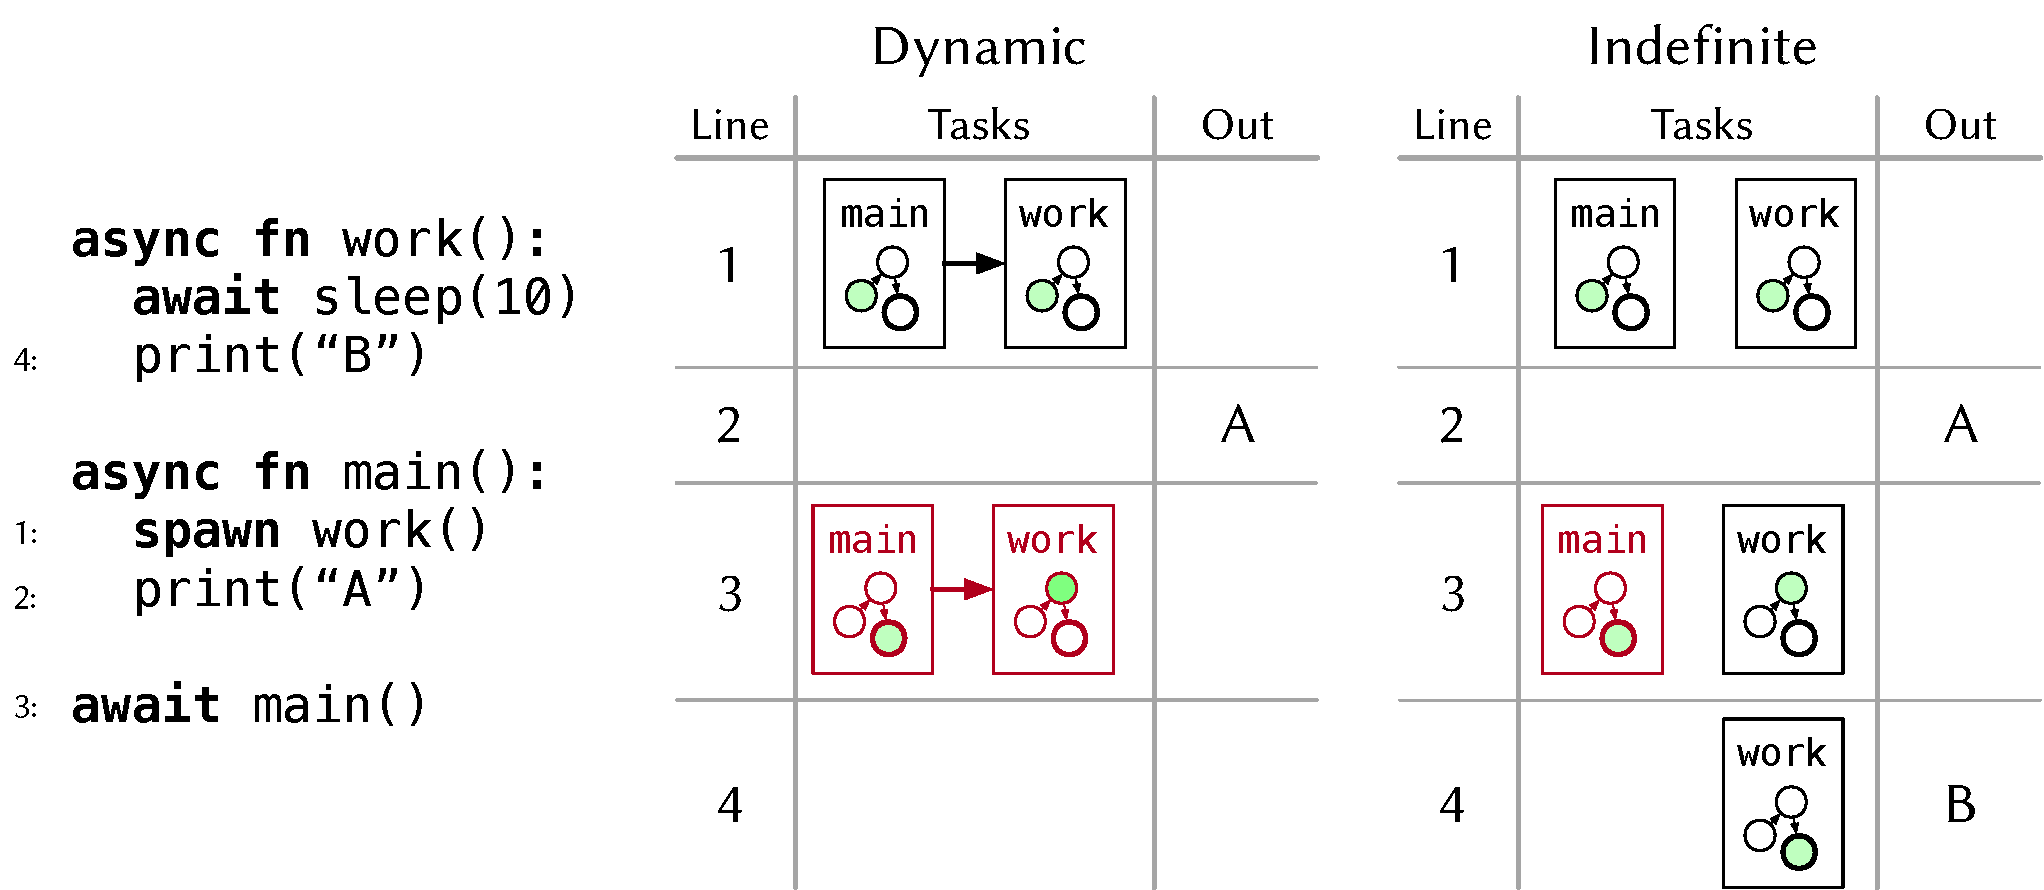
\includegraphics[width=0.82\linewidth]{./f/extent.pdf}
  \caption{An example program demonstrating the \extent dimension, executed with Swift (\dyn) and \Js (\indef). Each column shows the task structure and output after executing each line. Arrows between tasks indicate a parent-child relationship used for \dyn \extent.}
  \label{fig:extent}
\end{figure}

% \begin{figure}[t]
%   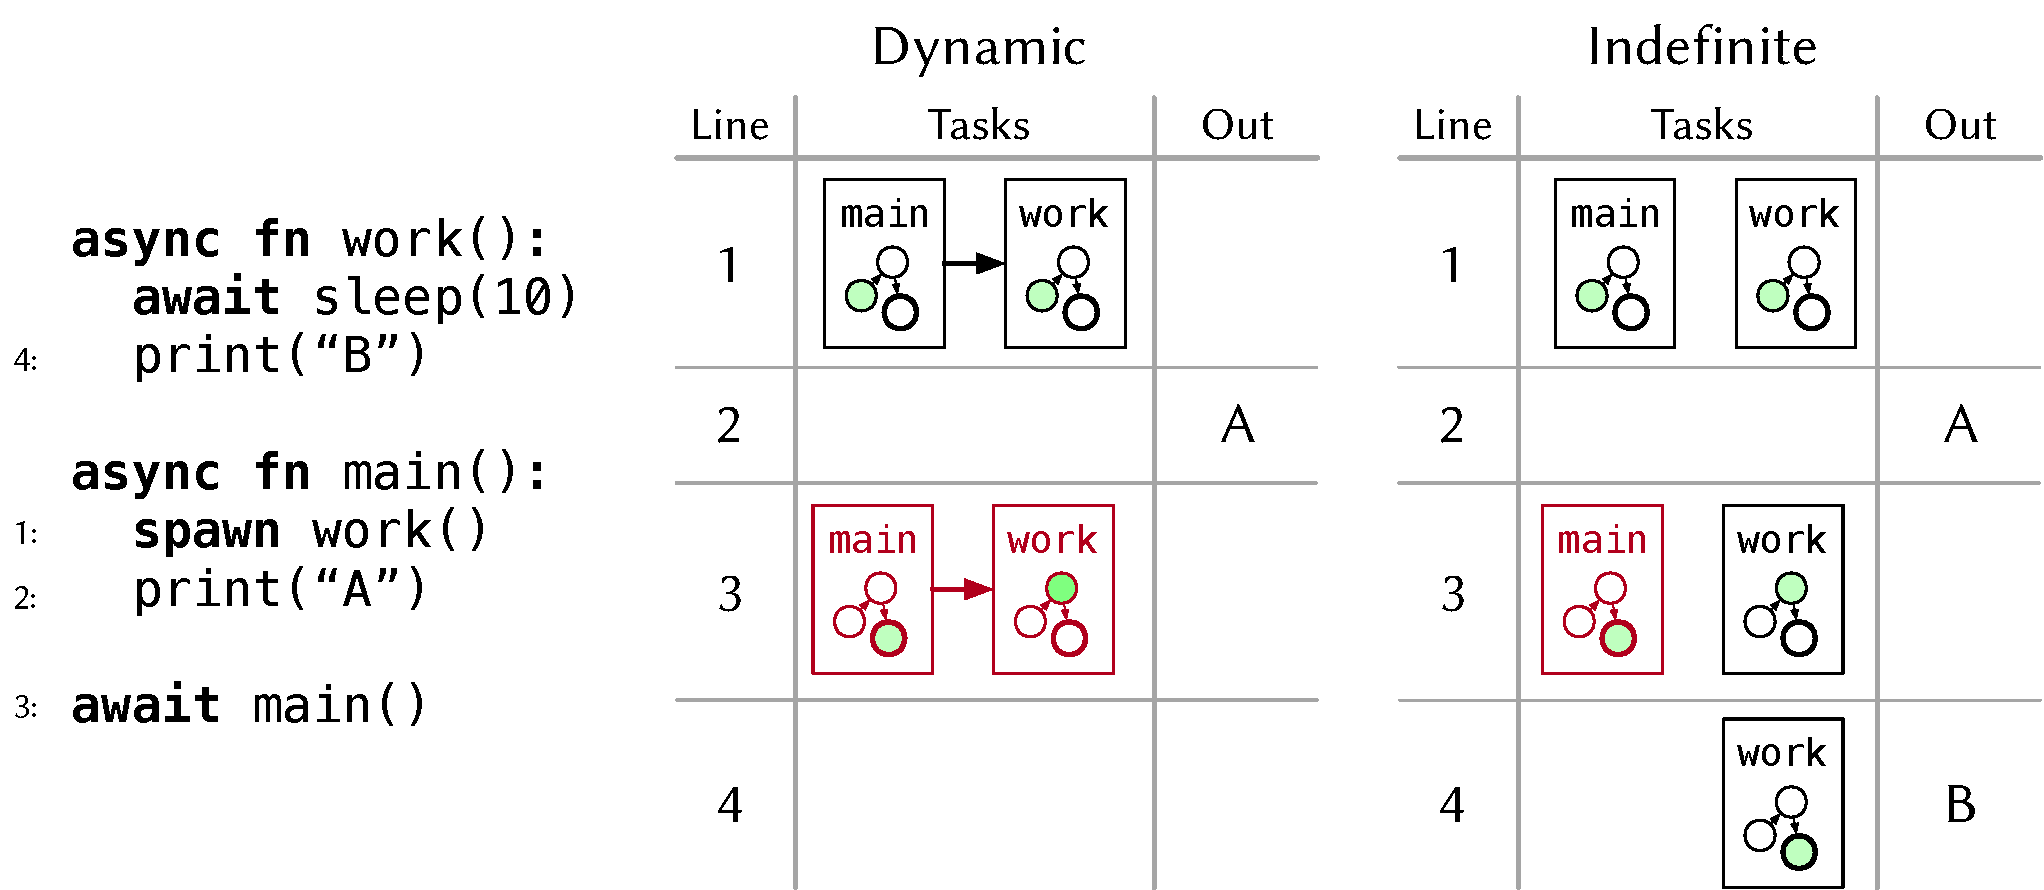
\includegraphics[width=0.7\linewidth]{./f/extent.pdf}
%   \caption{An example program demonstrating the \extent dimension, executed with Swift (\dyn) and \Js (\indef). Each column shows the task structure and output after executing each line. Arrows between tasks indicate a parent-child relationship used for \dyn \extent.}
%   \label{fig:extent}
% \end{figure}

Borrowing terminology from the Lisp community, the \extent of a task is the interval of time during which that task is capable of executing. For example, consider the program in \Cref{fig:extent}. What is the extent of the \code|spawn child_work()| task? The answer is it depends on quite a number of factors, as previously illustrated in \Cref{fig:motivating-example}.

In some designs for straight-line asynchrony, especially earlier designs, tasks by default have an \indef \extent: the task can live until it is no longer reachable, at which point the task is destructed. \Js, \CSharp, Python+Asyncio, and Rust+Tokio/Smol all use \indef \extent. Note that designs differ on how to determine reachability (see \Cref{ssec:designdims:references}), and designs also differ on the mechanism for destruction (see \Cref{ssec:designdims:destruction}). \Cref{fig:extent} illustrates \indef \extent, showing how the \code|child_work()| task outlives its parent \code|parent_work()| task, and the program waits until the work is completed.

Some have called \indef \extent an ``unstructured'' approach to asynchrony~\cite{smith_thoughts_2016}, akin to using goto for control flow, as task handles can easily go unhandled, leaving asynchronous work dangling with no clear policy for managing it.
%
This line of thought has led to the devleopment of ``structured'' asynchrony approaches~\cite{sustrik_structured_2025,mccall_swift_2021,elizarov_kotlin_2021}, which we describe as having \dyn \extent, found in Swift and Python+Trio. With \dyn \extent, a task's extent is tied to the extent of another task. In \Cref{fig:extent}, under \dyn \extent, the \code|child_work()| task is associated with the \code|parent_work()| task. When the \code|parent_work()| task completes, its associated tasks are destructed, which means cancellation in the case of Swift. Therefore the second print never occurs.

\paragraph{Design rationale.}

The main argument for \dyn \extent is that limiting tasks to known scopes leads to programs that are easier to reason about, and compose better with other language features~\cite{mccall_swift_2021,elizarov_kotlin_2021}. For instance in Python, \dyn \extent can ensure that a task within a \code|with| block will not use resources (e.g., file descriptors) after they have been cleaned up~\cite{smith_thoughts_2016}. However, existing implementations of \dyn \extent only support a strictly hierarchical model of parent-child task relationships (via \code|TaskGroup| in Swift and \code|Nursery| in Trio). These implementations disallow programs that might have more complex dependencies between tasks, such as two parent tasks awaiting the same child task.


\subsection{Reference Strength}\label{ssec:designdims:references}

The Runtime Reference Strength axis defines the strength of \task references held by the runtime. The possible values are: \textit{strong,} and \textit{weak.}

\begin{figure}[H]
  \begin{subfigure}[t]{0.49\textwidth}
\begin{lstlisting}[language=Rust]
use std::time::Duration;
use smol::Timer;
const sleep: fn(Duration) -> Timer =
  Timer::after;

async fn heartbeat() {
  loop {
    sleep(Duration::from_millis(1)).await;
    print!(".")
  }
}

async fn work() {
  let t = smol::spawn(heartbeat());
  sleep(Duration::from_millis(5)).await;
  print!("A");
}

fn main() {
  smol::block_on(async {
    work().await;
    print!("B");
    sleep(Duration::from_millis(5)).await;
  })
} // => "....AB"
\end{lstlisting}
    \cprotect\caption{An  example of  weak  runtime references. The SMOL (Rust) framework does not hold strong references to running \tasks. The program prints ``....AB'' with never any trailing periods after the `B.'}
    \label{fig:designdims:refs:weak}
  \end{subfigure}\hfill%
  \begin{subfigure}[t]{0.49\textwidth}
\begin{lstlisting}[language=Rust]
use std::time::Duration;
use tokio::time::sleep;



async fn heartbeat() {
  loop {
    sleep(Duration::from_millis(1)).await;
    print!(".")
  }
}

async fn work() {
  let t = tokio::spawn(heartbeat());
  sleep(Duration::from_millis(5)).await;
  print!("A");
}

#[tokio::main]
async fn main() {
  work().await;
  print!("B");
  sleep(Duration::from_millis(5)).await;
} // => "....AB...."
\end{lstlisting}
\cprotect\caption{An  example of  strong  runtime references. The Tokio (Rust) framework holds strong references to running \tasks. The program prints ``....AB....'' with some amount of trailing periods printed during the sleep within the \code{main} function.}
    \label{fig:designdims:refs:strong}
  \end{subfigure}
  \cprotect\caption{An example of weak and strong runtime references.}
  \label{fig:designdims:refs}
\end{figure}

The \task reference strength held by the runtime is important for systems with \textit{indefinite} \task extent (see \Cref{ssec:dims:extent}). Shown in \Cref{fig:designdims:refs:weak} the SMOL (Rust) system holds weak pointers to running \tasks.\footnote{The \code{.detach()} method can be invoked on \tasks to transfer ownership to the runtime system, turning the default weak references into strong references.} When no more references exist to the \task \code{t}, established on line 14, the \task is cancelled and deallocated. The output will have no trailing periods printed  because the heartbeat task is cancelled on line 17 when the reference \code{t} goes out of scope.

In contrast, the Tokio (Rust) system holds strong references to \tasks. The \task referenced by \code{t} is not destroyed when \code{t} goes out of scope, because the runtime continues to hold a reference to the \task. The output will contain some number of trailing periods after the `B,' as the heartbeat \task continues to execute while the main function sleeps on line 23.

Weak runtime references are used by SMOL (Rust) to prevent dangling \tasks from consuming resources without the devlopers knowledge. A \task is automatically cancelled and deallocated when no further references to it exist; a deterministic effect thanks to Rusts ownership type system. This behavior parallels the behavior of memory allocation in Rust. Asyncio (Python) also holds weak references to \tasks, which is a source of controversy in the ecosystem~\cite{hartl_asyncio_2022}. At the time of writing, Asyncio's use of weak references is marked as a bug, however, the community is hesitant to change the design without understanding why it was designed this way to begin with; a fact that is undocumented and not remembered by the core developers.


\subsubsection{\Destruction}\label{ssec:designdims:destruction} 

\begin{figure}[t]
  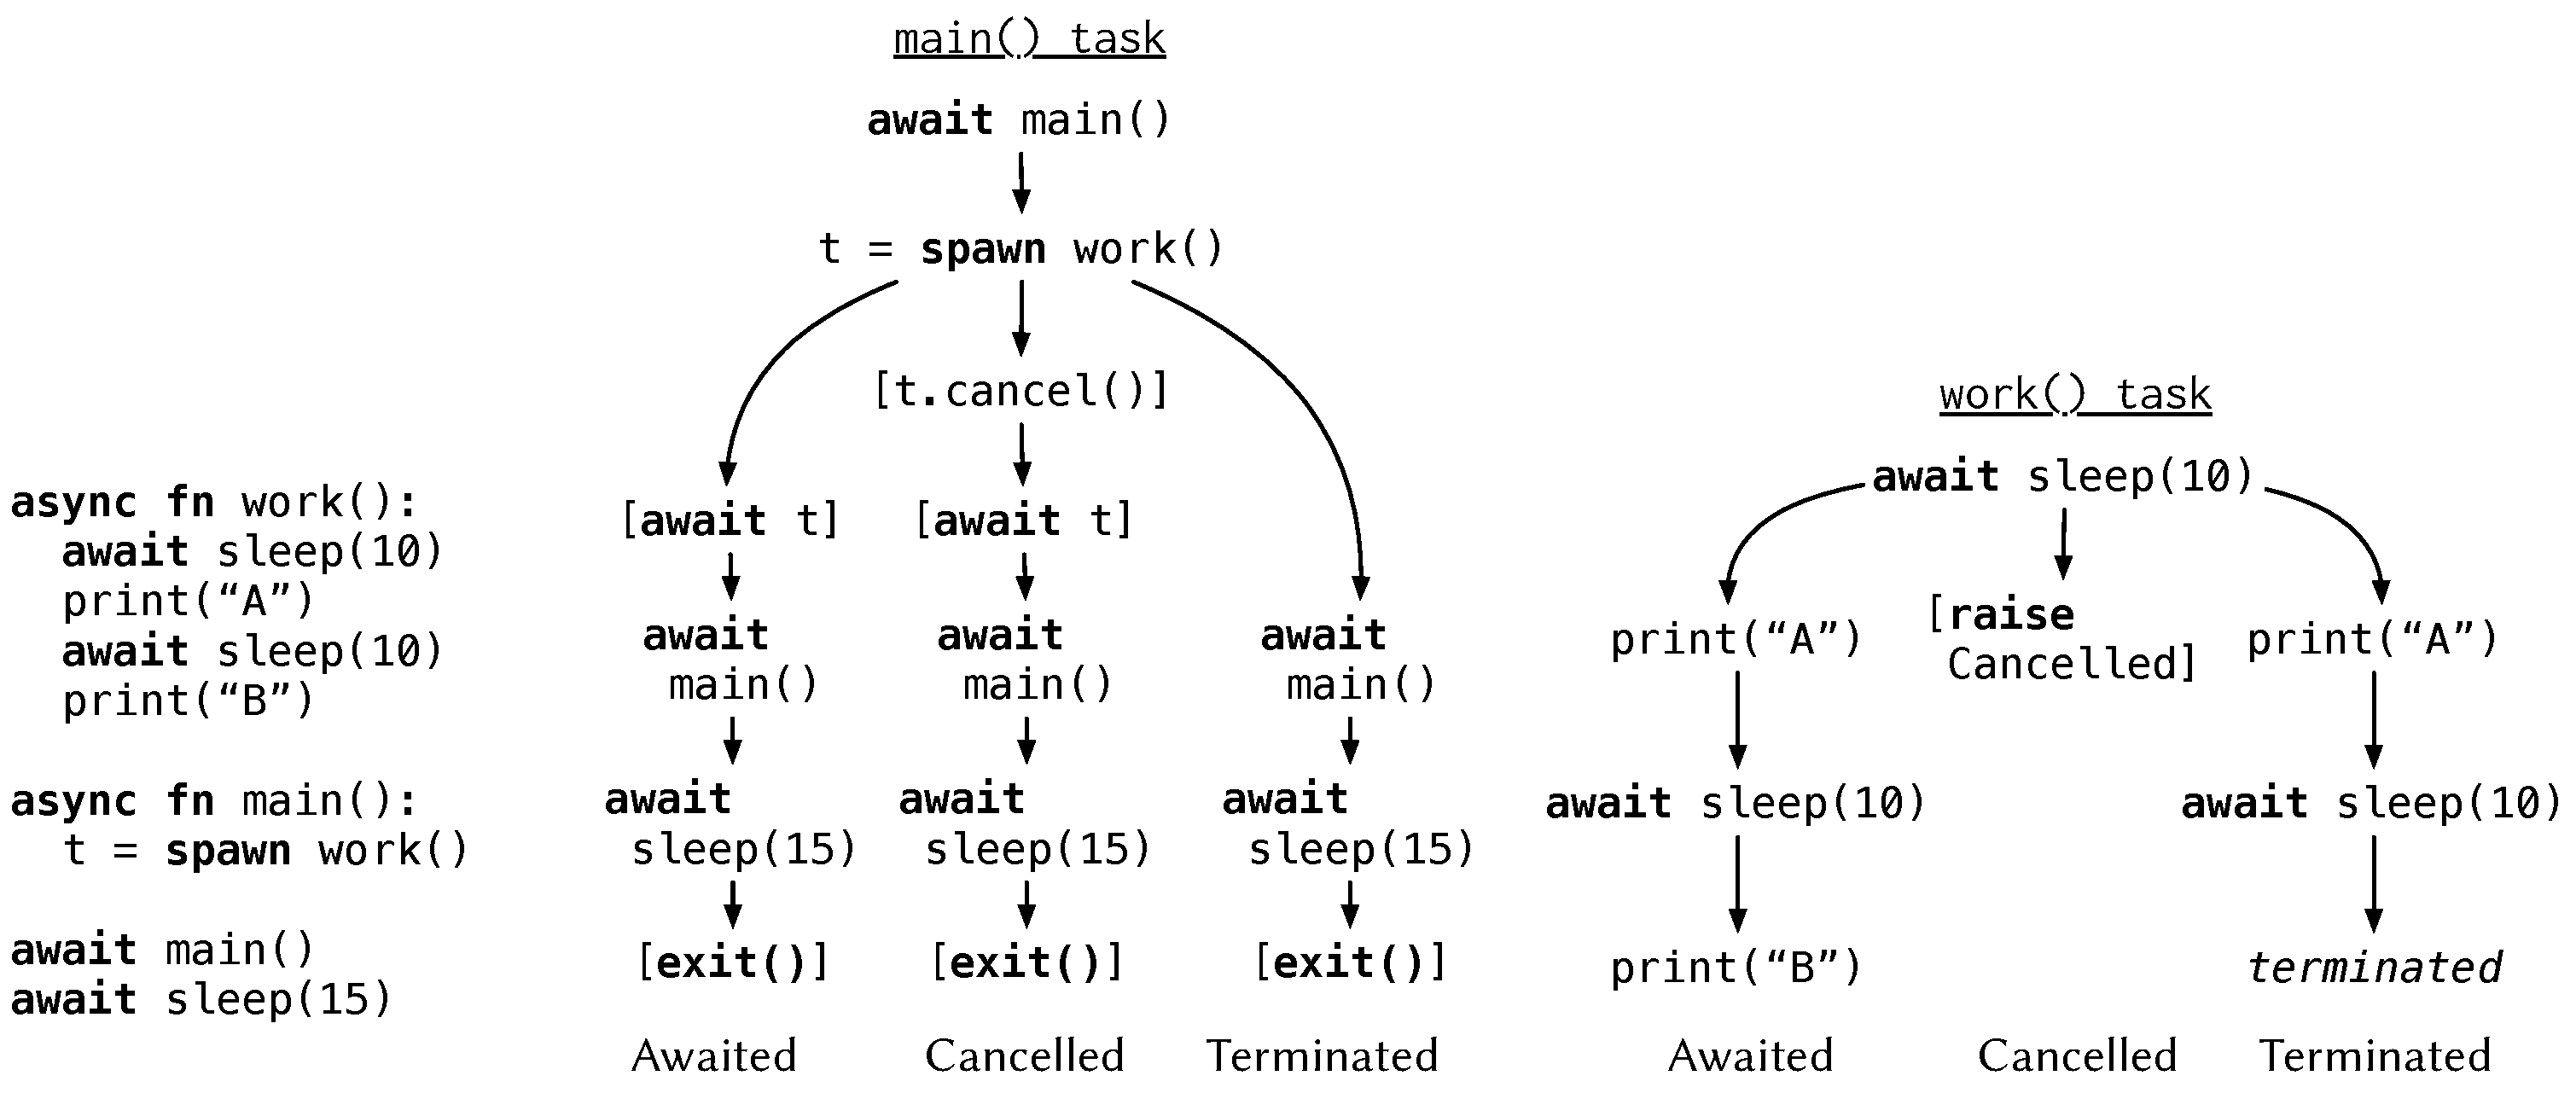
\includegraphics[width=\linewidth]{f/destruction.pdf}
  \caption{\Destruction [CAPTION TODO]}
  \label{fig:destruction}
\end{figure}


Once a language has decided that it is time to destruct a task, we encounter yet another point of divergence: what does it mean to destruct a task? For example, consider the program in \Cref{fig:destruction}. At the end of the \extent of the spawned \lstinline[language=Pseudo]|work()| task (either end of \lstinline[language=Pseudo]|main()| for \dyn \extent, or end of program for \indef \extent), what happens to the \lstinline[language=Pseudo]|work()| task? Today's languages offer three possibilities: to \emph{await} the task, to \emph{cancel} the task, and to \emph{terminate} the task.

The \destruction dimension is orthogonal to \extent. \Js is a language with \indef \extent and awaiting destruction --- \Cref{fig:extent} previously showed an example relying on this pair of design decisions. Python+Trio is a language/system with \dyn \extent and awaiting destruction, as tasks are tied to a ``nursery,'' and the nursery waits until all its child tasks are completed before exiting. The awaiting column in \Cref{fig:destruction} demonstrates Trio semantics, where the program would print ``ABC'' by waiting for the \lstinline[language=Pseudo]|work()| task to before exiting \lstinline[language=Pseudo]|main()|.

Most other designs opt to cancel tasks at the end of extent, such as Swift, Rust+Tokio, Rust+Smol, and Python+Asyncio. [TODO: ARE SMOL AND SWIFT ACTUALLY COMPARABLE?]


% The \Task Destruction axis defines what happens to a task when the \task object is destroyed by the system. The possible values are: \textit{awaited,} \textit{cancelled,} or \textit{terminated.}

% \Cref{fig:designdims:destruction:await} shows an example JavaScript program that awaits \tasks on destruction~\missingcite, even though there is no explicit \code{await} keyword. The program terminates after 10 seconds and prints ``exiting'' and ``done.''

% \Cref{fig:designdims:destruction:cancel} shows an example Swift program that cancels a running task on destruction~\missingcite. Because that task is executing a long sleep operation, the sleep is cancelled --- on cancellation \code{Task.sleep} raises an exception that we suppress with the \code{try?} keyword --- and the program continues executing. The program terminates after ~0.5 seconds and prints ``exiting,'' ``cancelled'' and ``done.''

% \Cref{fig:designdims:destruction:term} shows an example \CSharp program that terminates running \tasks on destruction~\missingcite. The program terminates after ~0.5 seconds and prints ``exiting.''

% Where your language falls on the destruction axis informs the safety and responsiveness of the system. Await destruction allows running \tasks to complete, which provides data/invariant integrity for the program at the expense of responsiveness.

% Cancel destruction may provide \tasks the chance to safely reclaim resources --- depending on the language's chosen cancellation semantics --- however, programs may still suffer from responsiveness issues if cancelling a \task requires the \task's cooperation. We discuss cancellation semantics in \Cref{ssec:designdims:cancellation}.

% Terminate destruction prioritizes speed over safety. A running \task may hold system resources or be in the middle of an operation, by cancelling the \task the system risks deadlocks and breaking logical invariants.


\subsubsection{\Propagation}\label{ssec:designdims:propagation}

\begin{wrapfigure}{r}{0.37\linewidth}
\begin{lstlisting}[language=Py]
from trio import open_nursery

async def fail():
  raise Exception()

async def main():
  print("A")
  async with open_nursery() as n:
    n.start_soon(fail)
  print("B")
\end{lstlisting}
  \cprotect\caption{An example of \destruct \propagation. Python+Trio reraises exceptions when their associated nursery scope ends.}
  \label{fig:propagation:trio}
\end{wrapfigure}

One final point of divergence at a task's end of life is the handling of exceptions. In all surveyed languages with exceptions (Python, Swift, \Js, \CSharp), awaiting on an async function that has thrown an exception will re-raise the exception at the await point.\footnotemark{} However, what happens to an exception raised in a task that is never awaited? We call this the \propagation dimension.%
\cprotect\footnotetext{Instead of exceptions Rust uses the \code|Result| type to communicate errors. An \code|Err| variant is returned on await, which we consider a semantically equivalent design to re-raising an exception at the await point.}

Most languages \never propagate, meaning the exception generates no behavior outside its containing task, apart from perhaps printing to the console. Python+Asyncio and \Js will print a stack trace for an uncaught asynchronous exception. Node.js\ specifically will exit with a non-zero error code, although this latter behavior is not part of the ECMAScript specification so we still categorize it as a \never approach to \propagation.

Python+Trio is the only system which offers a different semantics, in part because tasks cannot be awaited, so the library must offer another mechanism for observing asynchronous exceptions. The example in \Cref{fig:propagation:trio} (shown in Python, not pseudocode) will print ``A'' but not ``B'' because the nursery will re-raise the exception originating in the \code|fail| function. We describe this as \destruct \propagation. A similar program in any other system will print ``A'' then ``B'', possibly with a stack trace printed in-between.

\paragraph{Design rationale.} The upside to the \destruct approach is that an application is less likely to ignore problematic exceptions. With the \never approach, if a developer does not carefully monitor their logs, a task can fail and cause confusing bugs where expected operations never occur. 

The downside is that the \destruct approach may run counter to either a developer's intuitions (i.e., exceptions aren't thrown away by the system) or their desired software architecture. Concurrency \abbr{api}s often seek to encapsulate errors at thread or task boundaries, so errors in one thread cannot crash the whole system. For example, in a backend web server with many concurrent connections, it is likely undesirable that one exceptional connection should crash the entire server. Either way, it seems sensible that that a straight-line asynchrony \abbr{api} should offer \emph{some} way of accessing information about unawaited exceptions, rather than only printing to standard error, or ignoring unawaited exceptions outright.


\subsubsection{\Suspension}\label{ssec:designdims:suspension}

\begin{figure}[t]
  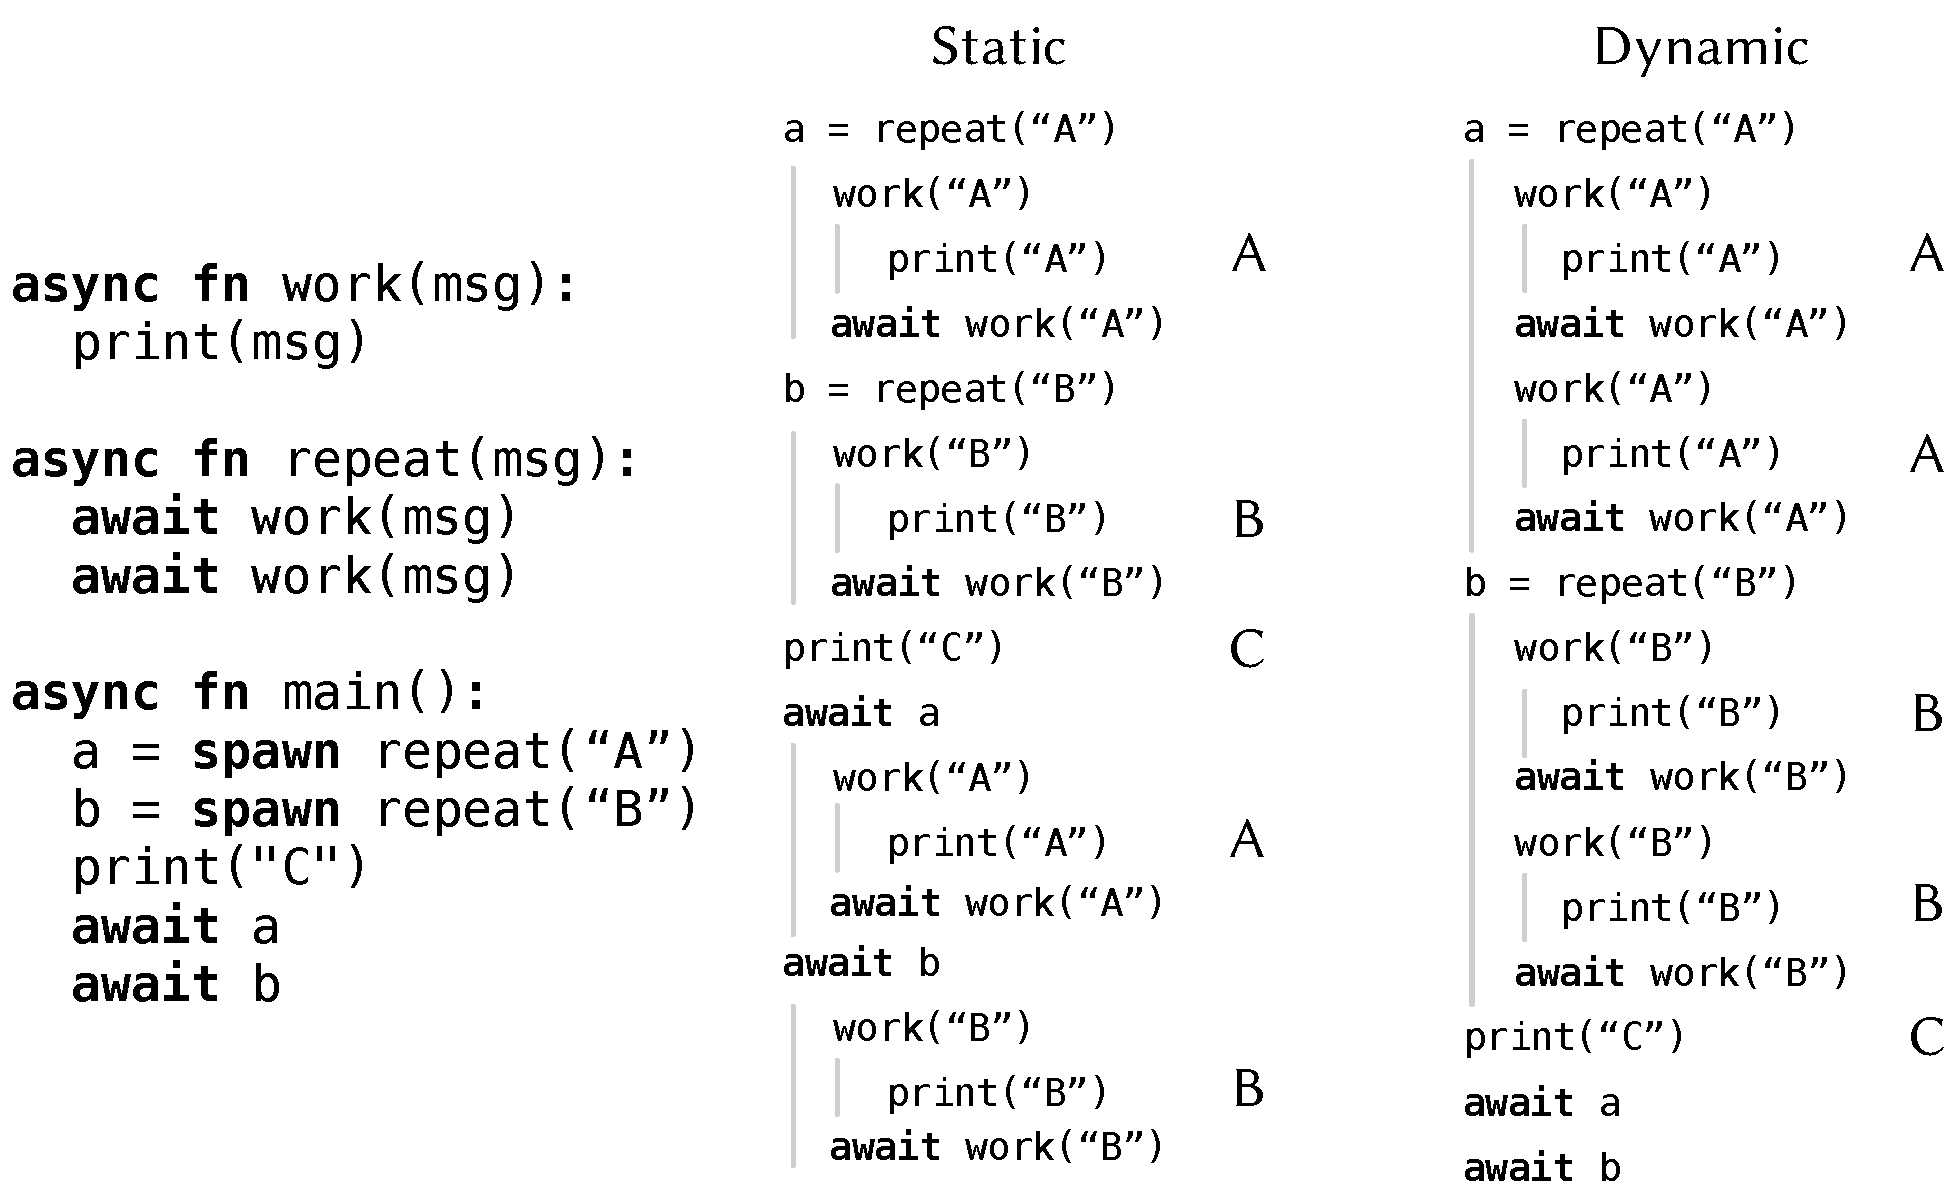
\includegraphics[width=0.7\linewidth]{f/suspension.pdf}
  \caption{An example program demonstrating the \Suspension dimension, executed with \Js (\static) and \CSharp (\dynamic). Each column shows an execution trace of the program under an eager semantics with each kind of \suspension. The execution traces are nested according to their level in the call stack, and the order of prints to stdout is emphasized in the right part of each column.}
  \label{fig:suspension}
\end{figure}

Once asynchronous work has started, the next design divergence occurs at await points. The \Suspension dimension defines the guarantees a language makes about whether an await point is guaranteed to yield control. For example, consider the program in \Cref{fig:suspension} executing under an \eager semantics. The line \code|a = repeat("A")| will call into \code|work("A")| which will call \code|print("A")| and return to \lstinline[language=Pseudo]|await work("A")|. The task for \code|work("A")| has been completed, so a language has two choices: either yield control to the caller, or continue evaluation past the \lstinline[language=Pseudo]|await|. We call the former strategy \emph{\static} suspension because an await point is statically guaranteed to always yield. We call the latter strategy \emph{\dynamic} suspension because whether an await point yields depends on the awaited task.

In only one language surveyed, \Js, an await point is guaranteed to yield according to the ECMAScript specification \cite[\textsection 27.7.5.3, step 3.b]{ecma_ecmascript_nodate}. Therefore in \Cref{fig:suspension}, running under \Js semantics, the program outputs ``ABCAB'' because \lstinline[language=Pseudo]|await work("A")| yields back to \code|main|. In all other languages, no such guarantee exists. For the example program operating under an eager semantics such as in \CSharp, the program would output ``AABBC'' because \lstinline[language=Pseudo]|await work("A")| observes that \code|work("A")| is complete and therefore the await expression can continue evaluation.

\paragraph{Design rationale.}

The principal reason to adopt \static suspension is to prevent starvation. Under an eager approach with \dynamic suspension, if a compute-bound task is called before calling \abbr{i/o}-bound tasks, the first task can starve the remaining tasks of CPU time. A \static suspension policy reduces the likelihood of that compute-bound task never yielding control back to the executor.

\Static suspension comes at a performance cost. In the case of awaiting a completed task, \static suspension requires a round-trip to the runtime and back to continue past the await. Languages with \dynamic suspension can mitigate the starvation issue by providing a \code|yield_now| primitive which has no effect but to yield control to the runtime.



\subsubsection{Cancellation} The Cancellation axis defines how a running task is cancelled, including how cancellation is signaled, if at all, and how cancellation propagates between task dependencies. A clear cancellation mechanism is what distinguishes async/await from other concurrency paradigms. Within the cancellation axis there are two design dimensions: \textit{cooperation,} and \textit{direction.}

\ggnote{This section has not been updated}

In this section we will illustrate cancellation using the function \code{process} defined in \Cref{fig:cancellation} in both Rust (SMOL) and Python (AsyncIO).

\begin{figure}
  \begin{minipage}[t]{0.49\textwidth}
\begin{lstlisting}[language=Rust, linebackgroundcolor={\lineEq{15}}]
async fn process(
  db: Database,
  cache: Cache,
  request: Request,
) -> Response {
  let response = compute_response(
    &db, &cache, request).await;

  let db_update = smol::spawn(
    update_db(&db, &response));

  let cache_update = smol::spawn(
    update_cache(&cache, &response));

    db_update.await;
    cache_update.await;

  response
}
  \end{lstlisting}
  \end{minipage}\hfill%
  \begin{minipage}[t]{0.49\textwidth}
\begin{lstlisting}[language=Python, linebackgroundcolor={\lineEq{11}}]
async def process(db, cache, request):
  response = await compute_response(
    db, cache, request)

  db_update = asyncio.create_task(
    update_db(db, response))

  cache_update = asyncio.create_task(
    update_cache(cache, response))

  await db_update
  await cache_update

  return response
\end{lstlisting}
  \end{minipage}
  \cprotect\caption{An illustrative async function, \code{process}, that processes a request, and in turn, updates a database and cache in parallel. It's important that the cache and database remain in sync, but the chosen cancellation policy may break this invariant. (Left) A Rust implementation using the SMOL async framework. SMOL uses a top-down, non-cooperative cancellation policy that may leave the database and cache in a \textit{partially-updated} state. (Right) A Python implementation using the Asyncio library. Asyncio uses a bottom-up, cooperative cancellation policy that may leave the database unchanged and the cache fully updated.}
  \label{fig:cancellation}
\end{figure}

\paragraph{Cooperation} The Cooperation cancellation axis defines if cancellation requires cooperation from all tasks in the cancelled subtree. If cancellation is \textit{cooperative,} this means that a cancellation signal can get intercepted by a node in the tree if they do not cooperate. Cancellation is \textit{non-}cooperative if tasks have no choice but to cooperate with cancellation; non-cooperative cancellation can otherwise be referred to as termination.

In Rust a \Coro{} is represented as an enumeration. Cancelling an \Coro{} is defined by simply freeing the value's memory. In the asynchronous framework SMOL, a \Task{} can be cancelled by either invoking the \code{.cancel()} method or freeing the \Task{}, which in turn frees the underlying \Coro{}. As a consequence of Rust's choice to define cancellation as a memory free, it is not possible for an asynchronous function to prevent a cancellation. A memory free cannot be shielded or intercepted. Therefore, we classify Rust's cancellation as non-cooperative. Note that this cancellation policy remains non-cooperative regardless of the async framework chosen for a specific program.

\begin{figure}
  \begin{minipage}[t]{0.49\linewidth}
    \includegraphics[width=0.99\textwidth]{example-image-a}
  \end{minipage}\hfill%
  \begin{minipage}[t]{0.49\linewidth}
    \includegraphics[width=0.99\textwidth]{example-image-b}
  \end{minipage}
  \cprotect\caption{Example execution of the \code{process} function shown in \Cref{fig:cancellation}. (Left) The Rust (SMOL) implementation uses the non-cooperative memory free cancellation protocol. Both the \code{db_update} and \code{cache_udpate} are terminated, leaving the systems in a potentially inconsistent state. (Right) The Python (Asyncio) implementation uses exceptions to signal cancellation and the \code{cache_update} is left orphaned because cancellation is not signaled to it.}
  \label{fig:cancellation:swimlane}
\end{figure}

Shown in \Cref{fig:cancellation:swimlane}, if the executing Rust function \code{process} is cancelled at line fifteen, then the memory for \code{process}, \code{db_update}, and \code{cache_update} are all freed. Neither the database update nor the cache update can rollback partially-made changes, so unless both operations completed fully before the cancellation, the system is left in an inconsistent state.

Cancellation in Python is handled by raising an exception at the next await point blocking the task. Refering to the code in \Cref{fig:cancellation}, if the \code{process} function is cancelled at line eleven, the exception will be raised at an await point within the \code{update_db} function. Because \code{process} is waiting on \code{db_update}, an await point blocking the task is within the dynamic extent of \code{update_db}. The \textit{expectation} is that \code{update_db} will allow the exception to propagate, or reraise the exception if it needs to do some cleanup.

\begin{wrapfigure}{r}{0.35\textwidth}
  \raggedright
\begin{lstlisting}[language=Python,numbers=none]
async def db_update(db r):
  snap = await db.snapshot()
  try:
    # .. cancelled in here ..
  except:
    await db_rollback(snap)
\end{lstlisting}
  \cprotect\caption{An example of a Python function swalling a cancellation request. The function \code{db_update} is not cooperating in the cancellation protocol by using a try/except block, which catches all exceptions.}
  \label{fig:cancellation:cooperative}
\end{wrapfigure}

The \code{db_update} function may choose to, or be mistakenly programmed to, not cooperate with cancellation. \Cref{fig:cancellation:cooperative} provides an illustrative implementation of the \code{db_update} function that does not cooperate with the Asyncio cancellation protocol. A \code{asyncio.CancellationError} will get raised within the \code{db_update} function, however, since the function body is wrapped in a try/except block, the cancellation request is never propagated to the \code{process} function. \code{process} is unaware that the database was not updated and the database and cache are now out of sync.

\paragraph{Propagation direction} The Propagation Direction axis defines where in the waiting tree of dependencies cancellation is signaled first and how that signal is propagated to the rest of the waiting nodes. The possible values are \textit{top-down,} \textit{bottom-up,} and \textit{simultaneous.}

Before specifying exactly what the direction of cancellation propagation is, we first need to specify through what cancellation is propagating. Cancellation propagates through the \textit{task tree,} specifically, the task tree rooted at the cancelled task. Not all languages explicitly build a task tree in the runtime.

Consider the Rust (SMOL) code in \Cref{fig:cancellation}, at line fifteen, the set of tasks is depicted in \Cref{fig:cancellation:tree:rust}. Unlike Python, an edge between two tasks in the SMOL task tree is added when a task is \textit{spawned,} not when it's awaited. We say this because the calling task has ownership of the spawned task. When a task is cancelled, SMOL invokes the destructors as they would typically run in Rust, which flows down the tree represented by memory ownership. Therefore, we say that Rust (SMOL) cancellation propagates top-down.

\begin{wrapfigure}{l}{0.30\linewidth}
  {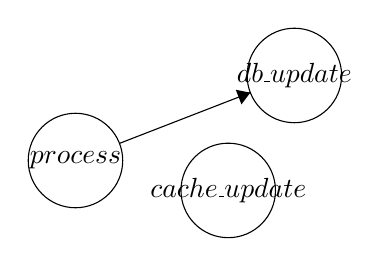
\begin{tikzpicture}[scale=0.2]
  \tikzstyle{every node}+=[inner sep=0pt]
    \draw [black] (13.3,-24.3) circle (3);
    \draw (13.3,-24.3) node {$\text{\tiny process}$};
    \draw [black] (27.2,-18.9) circle (3);
    \draw (27.2,-18.9) node {$\text{\tiny db\_update}$};
    \draw [black] (23,-26.2) circle (3);
    \draw (23,-26.2) node {$\text{\tiny cache\_update}$};
    \draw [black] (16.1,-23.21) -- (24.4,-19.99);
    \fill [black] (24.4,-19.99) -- (23.48,-19.81) -- (23.84,-20.74);
  \end{tikzpicture}
  \cprotect\subcaption{The state of the Python (Asyncio) task tree at line eleven. Because \code{process} is waiting on \code{db_update} the two form a tree, however, \code{cache_update} is not part of the current tree because it wasn't awaited.}
  \label{fig:cancellation:tree:python}}

  {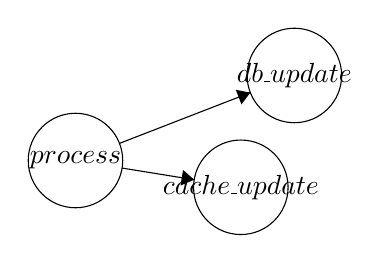
\begin{tikzpicture}[scale=0.2]
  \tikzstyle{every node}+=[inner sep=0pt]
  \draw [black] (13.3,-24.3) circle (3);
    \draw (13.3,-24.3) node {$\text{\tiny process}$};
  \draw [black] (27.2,-18.9) circle (3);
    \draw (27.2,-18.9) node {$\text{\tiny db\_update}$};
  \draw [black] (23.8,-26) circle (3);
    \draw (23.8,-26) node {$\text{\tiny cache\_update}$};
  \draw [black] (16.1,-23.21) -- (24.4,-19.99);
  \fill [black] (24.4,-19.99) -- (23.48,-19.81) -- (23.84,-20.74);
  \draw [black] (16.26,-24.78) -- (20.84,-25.52);
  \fill [black] (20.84,-25.52) -- (20.13,-24.9) -- (19.97,-25.89);
  \end{tikzpicture}
  \cprotect\subcaption{The state of the Rust (SMOL) task tree at line fifteen. Because SMOL's cancel on drop semantics, and Rust's owernship model, the task tree is help implicitly in Rust's memory.}
  \label{fig:cancellation:tree:rust}}

  \caption{The depicted task right before cancellation from the programs shown in \Cref{fig:cancellation}.}
  \label{fig:cancellation:tree}
\end{wrapfigure}

Consider the Python (Asyncio) code in \Cref{fig:cancellation}, at line 11, the set of tasks is depicted in \Cref{fig:cancellation:tree:python}. By default, all tasks in Asyncio are disjoint. Given two tasks, $A$ and $B$, where $B$ is spawned from within $A$, an edge in the task tree is added between the two nodes only when $A$ awaits $B$. Therefore, in our example program \code{db_update} is a child of \code{process} only because of the await present on line eleven. Therefore, cancellation is signalled from within \code{update_db}, and propagates \textit{upward} in the task tree to signal cancellation.

A \textit{simultaneous} cancellation would alert all tasks at the same time of cancellation. An example language with simultaneous cancellation propagation is Swift, as we will see in \Cref{sec:semantics}.



\subsection{Summary of Language Semantics}

\begin{table}
  \begin{tabular}{lllllll}
    \toprule
    System           & Eagerness   & Extent       & References   & Destruction  & Propagation  & Suspension  \\
    \midrule
    \CSharp          & eager       & indefinite   & strong  & terminated   & never        & dynamic     \\
    JavaScript       & eager       & indefinite   & strong  & awaited      & destruction  & static      \\
    Swift            & semi-eager  & dynamic      & -       & cancelled    & never        & dynamic     \\
    \midrule
    Tokio (Rust)     & lazy        & indefinite   & strong  & cancelled    & -            & dynamic     \\
    Smol (Rust)      & lazy        & indefinite   & weak    & cancelled    & -            & dynamic     \\
    \midrule
    AsyncIO (Python) & lazy        & indefinite   & weak    & terminated   & destruction  & dynamic     \\
    Trio (Python)    & lazy        & dynamic      & -       & awaited      & destruction  & dynamic     \\
    \bottomrule
  \end{tabular}
  \caption{Overview of semantic decisions make by language/system designers.}
  \label{tab:semantics-overview}
\end{table}

\begin{table}
  \begin{tabular}{lll}
    \toprule
    Language         & Cooperation      & Direction    \\
    \midrule
    Rust             & non-cooperative  & top-down     \\
    Swift            & cooperative      & simultaneous \\
    Python           & cooperative      & bottom-up    \\
    \bottomrule
  \end{tabular}
  \caption{Overview of cancellation decisions make by language/system designers}
  \label{tab:cancellation-overview}
\end{table}


\section{Semantics}\label{sec:semantics}

A key contribution of this paper is a precise and neutral description of the operational behavior of several contemporary async systems. To reduce the cosmetic noise we provide the operational semantics as extensions to a base $\lambda$-calculus variant, henceforth refered to as \lc. By providing the semantics in layers we highlight the control features necessary for a given language's implementation and can more easily compare the operational behavior between two languages that have seemingly incomparable semantics. We additionally provide all the semantics in this section as a runnable Redex model, available in the supplementary materials.~\missingcite

\begin{figure}[H]
  \begin{subfigure}[t]{0.39\textwidth}
    {$$
\begin{array}{r@{\ }c@{\ }l}
\mathsf{Number}\ n & & \mathsf{String}\ s \\
\mathsf{Const}\ c      & ::=  & \mathsf{true} \mid\mathsf{false}\mid n \mid s \\
\mathsf{Expr}\ e       & ::=  & x \mid v \mid \mathbfsf{fn}\ \many{x} \to e \mid e\ \many{e} \\
                       & \mid & \mathbfsf{let}\ x = e\ \mathbfsf{in}\ e \\
                       & \mid & \mathbfsf{if}\ e\ \mathbfsf{then}\ e\ \mathbfsf{else}\ e \\
                       & \mid & \mathbfsf{fix}\ e \mid e \mathbin{;} e \\
                       & \mid & \mathbfsf{reset}\ e \mid \mathbfsf{shift}\ x \to e \\
                       & \mid & \mathbfsf{ref}\ e \mid !e \mid e := e \\
\\
\mathsf{Value}\ v      & ::=  & c \mid () \mid \mathsf{ptr}(x) \\
       & \mid & \mathbfsf{fn}\ \many{x} \to e \mid \mathbfsf{fix}\ v \\
\\
\mathsf{Eval\ Ctx}\ E      & ::=  & [\cdot] \mid \many{v}\ E\ \many{e} \mid \mathbfsf{fix}\ E \\
       & \mid & \mathbfsf{let}\ x = E\ \mathbfsf{in}\ e \\
       & \mid & \mathbfsf{let}\ x = v\ \mathbfsf{in}\ E \\
       & \mid & \mathbfsf{if}\ E\ \mathbfsf{then}\ e\ \mathbfsf{else}\ e \\
       & \mid & \many{v} \mathbin{;} E \mathbin{;} \many{e} \mid \mathbfsf{reset}\ E \\
       & \mid & \mathbfsf{ref}\ E \mid !E \mid E := e \\
       & \mid & v := E
\\
\mathsf{Delim\ Ctx}\ M      & ::=\  & \mathsf{(} E\ \mathsf{without}\ \mathbfsf{reset}\ M \mathsf{)}
\\
\mathsf{Heap}\ \sigma & ::=  & \cdot \mid \sigma, x \mapsto v
\end{array}
$$

     \cprotect\caption{The grammar for \lc, a call-by-value variant of the $\lambda$-calculus with mutable references and delimited continuations.}
     \label{fig:lang:lc}}
  \end{subfigure}\hfill%
  \begin{subfigure}[t]{0.59\textwidth}
    {$$
\begin{array}{r@{\ }c@{\ }l}
  e & ::= \ldots \mid \bsfid{throw-in}\ e\ e\ \mid \bsfid{throw}\ e \mid \bsfid{try}\ e\ \bsfid{catch}\ e \\
  % \mathsf{Exn\ Ctx}\ G & ::=\  \mathsf{E} & \mid \bsfid{throw-in}\ e\ e\ \mid \bsfid{throw}\ e
\end{array}
$$

     \cprotect\subcaption{The grammar for \exn, which extends \lc with \code|try|/\code|catch|, and \code|throw| forms.}
    \label{fig:lang:exn}}
    \vspace{0.5em}
    {\noindent
\begin{tabular*}{\linewidth}{@{} l @{\extracolsep{\fill}} r @{}}
  $\langle \sigma, E[\bsfid{throw-in}(\mathbf{fn}\ x \to E_{\mathit{inner}}[x], v)] \rangle$ &  [Throw-In] \\
$\longrightarrow \langle \sigma, E[E_{\mathit{inner}}[\bsfid{throw}\ v]] \rangle$ &
\end{tabular*}

     \cprotect\subcaption{The operational semantics for the \exn.}
     \label{fig:lang:exn:red}}
  \end{subfigure}

  \caption{The syntax and semantics for the core \lc and \exn calculi.}
  \label{fig:lang:core}
\end{figure}

\Cref{fig:lang:core} provides the grammar and semantics of the core calculi that comprise our base for the async extensions. The core language \lc contains mutable references and delimited continuations via the \code|shift| and \code|reset| operators described by \citet{danvy_functional_nodate}. The grammar for \lc is provided in \Cref{fig:lang:lc}. The reduction rule is defined over a mutable heap $\sigma$ and an expression $e$, $\langle\sigma\,e\rangle$. The evaluation context $M$ is the continuation delimited by an enclosing \code|reset| form and captured by \code|shift|. For space reasons, the standard reduction rules and full grammar for \lc are available in \Cref{appendix}.

For languages with exceptional control flow, we extend \lc with a \code|try|/\code|catch| and \code|throw| form --- we will refer to this language as \exn. The grammar and reduction rules for \exn are provided in \Cref{fig:lang:exn}. The main contribution of this grammar is the evaluation context $G$, which is the exception context delimited by a \code|try| form and discarded by the \code|throw| operator. We also provide a \code|throw_in| expression that raises an exception within a suspended computation. We model this rule based on Python's \code{.throw()} coroutine method, which resumes a suspended computation with an exception instead of a value.

We now describe the configuration of the shared async grammar. \Cref{fig:lasync:grammar} defines the shared grammar constructs that encode the async runtime building blocks discussed in \Cref{sec:designdims}. We will refer to this shared grammar extension as the async platform, \lasync.

\begin{figure}[H]
  \begin{subfigure}[t]{\textwidth}
    $$
\begin{array}{l}
\begin{array}{rcl @{\hspace{3em}} rcl}
  \sfid{Time}\ t              & \in & \mathbb{N}_0 \cup \{\infty\}                              & \sfid{Frame}\ F         & ::= & \langle \ell, e \rangle \\
\sfid{Label}\ \ell          & ::= & x \mid \bsfid{sync}                    & \sfid{Frame\ Stack}\ FS & ::= & \epsilon \mid F \circ FS \\
\sfid{Continuation}\ \kappa & ::= & \bsfid{fn}\ x_{\mathit{unit}} \to e    & \sfid{Process}\ P       & ::= & \{ FS_1, \dots, FS_n \} \\
\sfid{Signal\ Queue}\ T     & ::= & \epsilon \mid (t, \ell, \kappa) \circ T & \sfid{Task\ Queue}\ Q   & ::= & \epsilon \mid (\ell, \kappa) \circ Q 
\end{array} \\
\\
\begin{array}{rcl}
e & ::= & \dots \mid \bsfid{sys-io}(e, e) \mid \bsfid{sys-start-soon}(\many{\ell,e}) \mid \bsfid{sys-start-later}(e, \ell, e)
% e & ::= & \dots \mid \bsfid{sys-block}(e) \mid \mathbfsf{sys-time}() \mid \mathbfsf{sys-io}(e, e) \mid \mathbfsf{sys-start-soon}(\many{\ell,e}) \mid \mathbfsf{sys-start-later}(e, \ell, e)
\end{array}
\end{array}
$$

    \cprotect\caption{The full grammar for \lasync.}
    \label{fig:lasync:grammar}
  \end{subfigure}\vspace{1em}
  \begin{subfigure}[t]{\textwidth}
    \begin{tabular*}{\linewidth}{@{} l @{\extracolsep{\fill}} r @{}}
  $\langle t, \sigma_0, Q, T, P \uplus \{ \langle \ell, E[\text{os\_io}(t_{\mathit{delay}}, v)] \rangle \circ FS \} \rangle$ & [OS-IO] \\
  $\longrightarrow \langle \text{step}(t), \sigma_1, Q, T, P \uplus \{ F_{\mathit{new}} \circ \langle \ell, E[x_{\mathit{io}}] \rangle \circ FS \} \rangle$ & \\
\multicolumn{2}{@{}l@{}}{
  $\begin{array}{l}
  \textbf{where } (\sigma_1, x_{io}) = \text{task\_alloc}(\sigma_0) \\
  \qquad e_{try} = \mathbfsf{try}\ none \mathbin{;} \text{task\_set\_done}(x_{io}, v)\ \mathbfsf{catch}\ e_{err} \to \text{task\_set\_failed}(x_{io}, e_{err}) \\
  \qquad e_{done} = e_{\mathit{try}} \mathbin{;} \text{os\_start\_soon}(\text{task\_get\_dependents}(x_{io})) \\
  \qquad F_{new} = \langle x_{\mathit{io}}, \text{os\_start\_later}(\text{os\_time}() + t_{\mathit{delay}}, x_{\mathit{io}}, \text{fun } () \to e_{done}) \rangle
  \end{array}$
}
\end{tabular*}

    \cprotect\caption{An example of the reduction rules for \lasync.}
    \label{fig:lasync:red}
  \end{subfigure}
  \caption{Syntax and state components for the Async Platform Language extension.}
  \label{fig:lasync}
\end{figure}

A \textit{frame}, $F$, is written $\langle \ell,\,e\rangle$ and consists of an expression $e$, along with a frame label, $\ell$. A \textit{frame label}, $\ell$, is either the name of the \task this frame corresponds to, or \textit{sync} to denote a synchronous frame. A \textit{frame stack}, $FS$, is a list of frames --- essentially a thread. An empty frame stack is written $\epsilon$, and we write $F \circ FS$ to denote a frame stack whose head is $F$ and tail is $FS$. A \textit{process}, $P$, is a collection of frame stacks. We will use the syntax $P \uplus FS$ to select one frame stack in $P$ to run. A \textit{task queue}, $Q$, stores the async work waiting to be run; $Q$ comprises tuples that have a label and a continuation, $(\ell,\kappa)$. A \textit{signals queue}, $T$, stores async work that is waiting on \abbr{io} operations, the work will be rescheduled in the future at timestampt $t$, at the earliest. $T$ comprises tuples that have a time, a label, and a continuation, $(t,\ell,\kappa)$. We will use the same stack notation for $Q$ and $T$ as we do for $FS$, but will write $Q \qpush (\ell,\,\kappa)$, and similarly for $T$, to append to the end of the queue.

The async platform provides a few additional expressions that we will describe here. The $\text{os\_block}\,e$ expression provides the barrier between synchronous code and asynchronous code. Languages may use a block expression to block a synchronous frame until the asynchronous expression has completed running. The block expression marks the runtime entry, and when it returns, the runtime exit.

The expression \code|os_io|$(e_t,e)$ is the \textsc{OmniScient io} operation provided by the runtime system. It models real-world \abbr{io} operations that would take some non-deterministic amount of time to resolve, like receiving packets from the network or querying a database. The form is omniscient because the resulting expression is provided upfront, e.g., \code|os_io|$(5, \text{``hello''})$ creates a \task that will resolve to the value ``hello'' after at least five time steps. Thus the form is deterministic in its evaluation \textit{value}, but not in its evaluation \textit{time.}

The expression \code|os_start_soon|$(\ell,\kappa)$ appends the continuation $\kappa$ to $Q$, set to run in a frame with the specified label $\ell$. The expression \code|os_start_later|$(t,\ell,\kappa)$ appends the continuation to the signal queue, $T$, which will be scheduled after timestep $t$. The expression \code|os_time|$()$ simply evaluates to the current timestep. 

The reduction rules for \lasync, and all languages that extent it, are defined over the tuple $\langle t, \sigma, Q, T, P \rangle$. The goal of the operational semantics is to highlight the differences between languages. As such we will present the same reduction rule from different languages together. We will also call attention to the portion of the redcution relevant to each design dimension with a highlight in the following colors: \ceag{\eagerness,} \cext{\extent,} \crfe{\references,} \cdes{\destruction,} \cpro{\propagation,} \csus{\suspension,} and \ccan{\cancellation.} We simply the presentation with a liberal use of metafunction; the full definitions of grammars, reductions, and metafunctions are provided in \Cref{app:semantics}.

\subsection{Async Function Application}

\begin{figure}[H]
  \noindent
$\begin{array}[t]{@{}r@{\ }l@{}l@{}l@{}l@{}}
                & \elided{\sigma_0, P \uplus \{ & & \langle \ell, E[(\bsfid{async\ fn}\ \many{x} \to e_{\mathit{body}})\ \many{v}] \rangle & {}\circ FS \}} \\
\longrightarrow & \elided{\sigma_2, P \uplus \{ \ceag{\langle x_{\mathit{task}}, e_{\mathit{task}} \rangle} & {}\circ{} & \langle \ell, E[x_{\mathit{task}}] \rangle & {}\circ FS \}}
\end{array}$\hfill$\text{[\CSharp/\Js-Async-App]}$\par
\begin{tabular*}{\linewidth}{@{} l @{\extracolsep{\fill}} r @{}}
\multicolumn{2}{@{}l@{}}{
  $\begin{array}{l}
  \where\ \many{x}_{\mathit{fresh}} = \many{\sfid{gensym}(),~ \sigma_1 = \sigma_0[\many{x}_{\mathit{fresh}} \mapsto \many{v}],~ e_{\mathit{subst}} = e_{\mathit{body}}[\many{x}_{\mathit{fresh}}/\many{x}]} \\
  \qquad (\sigma_2, x_{\mathit{task}}) = \sfid{task-alloc}(\sigma_1)\;\cext{\ghost} \\
  \qquad e_{\mathit{task}} = \bsfid{reset}\ ( \\
  \qquad \qquad \bsfid{try}\ \semmacro{task-set-done}(x_{\mathit{task}}, e_{\mathit{subst}})\ \bsfid{catch}\ v_{\mathit{err}} \to \semmacro{task-set-failed}(x_{\mathit{task}}, v_{\mathit{err}}) \\
  \quad\;\;\cdes{\ghost}\;\cext{\ghost}\;\cpro{\ghost}\;
  \bsfid{sys-start-soon}(\semmacro{task-get-dependents}(x_{\mathit{task}})))
  \end{array}$
}
\end{tabular*}

\vspace{1em}
\noindent
$\begin{array}[t]{@{}r@{\ }l@{\ }l@{}l@{}}
                & \elided{\sigma_0, Q, & P \uplus \{ \langle \ell, E[(\bsfid{async\ fn}\ \many{x} \to e_{\mathit{body}})\ \many{v}] \rangle & {}\circ FS \}} \\
\longrightarrow & \elided{\sigma_3, \ceag{Q \qpush (x_{\mathit{task}}, \kappa)}, & P \uplus \{ \langle \ell, E[x_{\mathit{task}}] \rangle & {}\circ FS \}}
\end{array}$\hfill$\text{[Swift-Async-App]}$\par
\begin{tabular*}{\linewidth}{@{} l @{\extracolsep{\fill}} r @{}}
\multicolumn{2}{@{}l@{}}{
  $\begin{array}{l}
  \where\ \many{x}_{\mathit{fresh}} = \many{\sfid{gensym}(),~ \sigma_1 = \sigma_0[\many{x}_{\mathit{fresh}} \mapsto \many{v}],~ e_{\mathit{subst}} = e_{\mathit{body}}[\many{x}_{\mathit{fresh}}/\many{x}]} \\
  \qquad (\sigma_2, x_{\mathit{task}}) = \sfid{task-alloc}(\sigma_1) \\
  \qquad \cext{\sigma_3 = \sfid{task-add-dependency}(\sigma_2, \ell, x_{\mathit{task}})} \\
  \qquad e_{\mathit{task}} = \bsfid{reset}\ ( \\
  \qquad \qquad \bsfid{try}\ \semmacro{task-set-done}(x_{\mathit{task}}, e_{\mathit{subst}})\ \bsfid{catch}\ v_{\mathit{err}} \to \semmacro{task-set-failed}(x_{\mathit{task}}, v_{\mathit{err}}) \mathbin{;} \\
  \qquad \qquad \cdes{\semmacro{task-cancel-dependencies}(x_{\mathit{task}}) \mathbin{;}} \\
  \qquad \qquad \cext{\semmacro{task-wait-on-dependencies}(x_{\mathit{task}}) \mathbin{;}}\;\cpro{\ghost}\\
  \qquad \qquad \bsfid{sys-start-soon}(\semmacro{task-get-dependents}(x_{\mathit{task}}))) \\
  \qquad \kappa = \bsfid{fn}\ x_\mathit{unit} \to x_\mathit{unit}\mathbin{;}\ e_{\mathit{task}}
  \end{array}$
}
\end{tabular*}

\vspace{1em}
\noindent
$\begin{array}[t]{@{}r@{\ }l@{}}
                & \langle \sigma_0, E[(\bsfid{async\ fn}\ \many{x} \to e_{\mathit{body}})\ \many{v}] \rangle \\
\longrightarrow & \langle \sigma_1, E[\ceag{\bsfid{reset}\ (\bsfid{shift}\ k \to k \mathbin{;} e_{\mathit{subst}})}] \rangle
\end{array}$\hfill$\text{[Rust/Python-Async-App]}$\par
\begin{tabular*}{\linewidth}{@{} l @{\extracolsep{\fill}} r @{}}
\multicolumn{2}{@{}l@{}}{
  $\begin{array}{l}
  \where\ \many{x}_{\mathit{fresh}} = \many{\sfid{gensym}(),~ \sigma_1 = \sigma_0[\many{x}_{\mathit{fresh}} \mapsto \many{v}],~ e_{\mathit{subst}} = e_{\mathit{body}}[\many{x}_{\mathit{fresh}}/\many{x}]}
  \end{array}$
}
\end{tabular*}

  \makelegend{eag,ext,ref,des,pro,sus,can}
  \cprotect\caption{A comparison of the rule \semrule{Async-App} across languages.}
  \label{fig:async-app}
\end{figure}

\Cref{fig:async-app} shows the \semrule{Async-App} rule for \CSharp, Swift, and Python; the rule primarily has implications for \eagerness. In \CSharp a new \task is allocated, the function body, which is placed inside error handling logic to trap exceptions, is set in a new frame on the \emph{top} of the current frame stack. After the entire body has run and a value set in the \task, the dependents of the \task are rescheduled in the task queue. Note that dependencies of the \task are not waited on, cancelled, or terminated as they have indefinite extent.

The \semrule{Async-App} rule for Swift follows a similar procedure as that of \CSharp's, but with several important changes. First, the \task allocated is not independent, it is a \emph{dependency} of the currently executing \task labelled $\ell$. Registering spawned \tasks as dependencies is important because at the end of execution a \task will cancel and wait on it's dependencies before rescheduling its dependents in the task queue. Note that dependencies are \emph{waited on} and not \emph{awaited,} by merely waiting on dependencies to finish, any errors that occur are not propagated. The second key difference is that the newly created \task is appended to the task queue, not placed on the current frame stack.

\begin{figure}[H]
  \noindent
$\begin{array}[t]{@{}r@{\ }l@{\ }l@{}l@{}}
                & \elided{ \sigma_0, Q, & P \uplus \{ \langle \ell, E[\bsfid{spawn}\ v_{\mathit{coro}}] \rangle & {}\circ FS \}} \\
\longrightarrow & \elided{ \sigma_1, \ceag{Q \qpush (x_{\mathit{task}}, \kappa)}, & P \uplus \{ \langle \ell, E[x_{\mathit{task}}] \rangle & {}\circ FS \}}
\end{array}$\hfill$\text{[Asyncio/Tokio/Smol-Spawn]}$\par
\begin{tabular*}{\linewidth}{@{} l @{\extracolsep{\fill}} r @{}}
\multicolumn{2}{@{}l@{}}{
  $\begin{array}{l}
  \where\ (\sigma_1, x_{\mathit{task}}) = \sfid{task-alloc}(\sigma_0) \\
  \qquad e_{\mathit{task}} = \bsfid{reset}\ ( \\
  \qquad \qquad \difff{\bsfid{try}}\ \semmacro{task-set-done}(x_{\mathit{task}}, \bsfid{await}\ v_{\mathit{coro}})\ \difff{\bsfid{catch}\ v_{\mathit{err}} \to \semmacro{task-set-failed}(x_{\mathit{task}}, v_{\mathit{err}})} \mathbin{;} \\
  \quad\;\;\cdes{\ghost}\;\cext{\ghost}\;\cpro{\ghost}\;
  \bsfid{sys-start-soon}(\semmacro{task-get-dependents}(x_{\mathit{task}}))) \\
  \qquad \kappa = \bsfid{fn}\ x_{\mathit{unit}} \to x_{\mathit{unit}} \mathbin{;} e_{\mathit{task}}
  \end{array}$
}
\end{tabular*}

\vspace{1em}
\noindent
$\begin{array}[t]{@{}r@{\ }l@{\ }l@{}l@{}}
                & \elided{ \sigma_0, Q, & P \uplus \{ \langle \ell, E[\bsfid{spawn}\ v_{\mathit{coro}}] \rangle & {}\circ FS \}} \\
\longrightarrow & \elided{ \sigma_2, \ceag{Q \qpush (x_{\mathit{task}}, \kappa)}, & P \uplus \{ \langle \ell, E[x_{\mathit{task}}] \rangle & {}\circ FS \}}
\end{array}$\hfill$\text{[Trio-Spawn]}$\par
\begin{tabular*}{\linewidth}{@{} l @{\extracolsep{\fill}} r @{}}
\multicolumn{2}{@{}l@{}}{
  $\begin{array}{l}
  \where\ (\sigma_1, x_{\mathit{task}}) = \sfid{task-alloc}(\sigma_0) \\
    \qquad \cext{\sigma_2 = \sfid{task-add-dependency}(\sigma_1, \ell, x_{\mathit{task}})} \\
  \qquad e_{\mathit{task}} = \bsfid{reset}\ ( \\
  \qquad \qquad \bsfid{try}\ \semmacro{task-set-done}(x_{\mathit{task}}, \bsfid{await}\ v_{\mathit{coro}})\ \bsfid{catch}\ v_{\mathit{err}} \to \semmacro{task-set-failed}(x_{\mathit{task}}, v_{\mathit{err}}) \mathbin{;} \\
  \qquad \quad\;\cdes{\ghost}\;\cext{\semmacro{task-wait-on-dependencies}(x_{\mathit{task}}) \mathbin{;}}\\
  \qquad \qquad \cpro{\semmacro{task-reraise-dependency-failures}(x_{\mathit{task}}) \mathbin{;}} \\
  \qquad \qquad \bsfid{sys-start-soon}(\semmacro{task-get-dependents}(x_{\mathit{task}}))) \\
  \qquad \kappa = \bsfid{fn}\ x_{\mathit{unit}} \to x_{\mathit{unit}} \mathbin{;} e_{\mathit{task}}
  \end{array}$
}
\end{tabular*}

  \makelegend{eag,ext,ref,des,pro,sus,can}
  \cprotect\caption{A comparison of \semrule{Spawn} across Python runtimes.}
  \label{fig:spawn}
\end{figure}

The rule \semrule{Async-App} for Python is compared to the others very simple. Python's async design separates the \coro mechanism --- generated by the compiler from an \psudo{async} function --- and the runtime. Because Python exposes \coros as a building block for runtime libraries, an async function application evaluates immediately to a \coro. To compare the lifecycles of \tasks between languages the rules \semrule{Spawn} for Asyncio and Trio are included in \Cref{spawn}. An important detail in the definitions for \semrule{Spawn} is Trio's enforcement of \dyn \extent. In Trio, when a \task finishes executing it will \emph{await} its dependencies without cancelling them.

\ggnote{TODO PICK UP HERE: I caved and decided that SK's suggestion for presenting the semantics was better}

\subsection{\CSharp}

\begin{figure}[H]
  \begin{subfigure}{\textwidth}
    $$
\begin{array}{rcl @{\hspace{3em}} rcl}
  e & ::= & \ldots \mid \mathbfsf{async\ fn}\ \many{x} \to e \mid \mathbfsf{await}\ e & v & ::= & \ldots \mid \mathbfsf{async\ fn}\ \many{x} \to e
\end{array}
$$

    \cprotect\caption{The grammar extension for \CSharp's async/await expressions.}
    \label{fig:cs:grammar}
  \end{subfigure}\vspace{1em}
  \begin{subfigure}{\textwidth}
    \noindent
\begin{tabular*}{\linewidth}{@{} l @{\extracolsep{\fill}} r @{}}
$\langle t, \sigma_0, Q, T, P \uplus \{ \langle \ell, E[(\mathbf{async\ fn}\ \many{x} \to e_{\mathit{body}})\ \many{v}] \rangle \circ FS \} \rangle$ & [Async-App] \\
$\longrightarrow \langle \mathrm{step}(t), \sigma_2, Q, T, P \uplus \{ \ceag{F_{\mathit{new}}} \circ \langle \ell, E[x_{\mathit{task}}] \rangle \circ FS \} \rangle$ & \\
\multicolumn{2}{@{}l@{}}{
  $\begin{array}{l}
  \textbf{where}\\
  \qquad (\sigma_1, x_{\mathit{task}}) = \mathrm{task\_alloc}(\sigma_0)\ \mathrm{and}\ \many{x}_{\mathit{fresh}} = \many{\mathrm{gensym}()} \\
  \qquad \sigma_2 = \sigma_1[\many{x}_{\mathit{fresh}} \mapsto \many{v}] \\
  \qquad e_{\mathit{subst}} = e_{\mathit{body}}[\many{x}_{\mathit{fresh}}/\many{x}] \\
  \qquad e_{\mathit{try}} = \mathbfsf{try}\ \mathrm{task\_set\_done}(x_{\mathit{task}}, e_{\mathit{subst}})\ \mathbfsf{catch}\ v_{\mathit{err}} \to \mathrm{task\_set\_failed}(x_{\mathit{task}}, v_{\mathit{err}}) \\
  \qquad F_{\mathit{new}} = \langle x_{\mathit{task}}, \mathrm{reset}\ (e_{\mathit{try}} \mathbin{;} \cext{\mathrm{os\_start\_soon}(\mathrm{task\_get\_dependents}(x_{\mathit{task}}))}) \rangle
  \end{array}$
}
\end{tabular*}

\vspace{1.5em}

\noindent
\begin{tabular*}{\linewidth}{@{} l @{\extracolsep{\fill}} r @{}}
$\langle t, \sigma, Q, T, P \uplus \{ \langle \ell, E[\mathbf{await}\ v_{\mathit{aw}}] \rangle \circ FS \} \rangle$ & [Await] \\
$\longrightarrow \langle \mathrm{step}(t), \sigma, Q, T, P \uplus \{ \langle \ell, E[e_{\mathit{check}}] \rangle \circ FS \} \rangle$ & \\
\multicolumn{2}{@{}l@{}}{
  $\begin{array}{l}
    \textbf{where}\\
   \qquad e_k = \mathrm{shift}\ k \to \mathrm{task\_add\_self\_as\_dependent}(v_{\mathit{aw}}, \ell,\mathrm{task\_continue\_with}(v_{\mathit{aw}},k)) \\
  \qquad e_{\mathit{check}} = \csus{\mathrm{if}\ \mathrm{task\_is\_completed}(v_{\mathit{aw}})\ \mathrm{then}\ \mathrm{task\_get\_result}(v_{\mathit{aw}})\ \mathrm{else}\ e_k}
  \end{array}$
}
\end{tabular*}

\vspace{1.5em}

\noindent
\begin{tabular*}{\linewidth}{@{} l @{\extracolsep{\fill}} r @{}}
$\langle t, \sigma, Q, T, P \uplus \{ \langle \mathrm{root}, E[\mathrm{os\_block}\ v_{\mathit{aw}}] \rangle \circ FS \} \rangle$ & [OS-Block-Done] \\
$\longrightarrow \langle \mathrm{step}(t), \sigma, \cdes{\epsilon}, \cdes{\epsilon}, \{ \langle \mathrm{root}, E[\mathrm{task\_get\_result}(v_{\mathit{aw}})] \rangle \circ \cdes{\epsilon} \} \rangle$ & \\
\multicolumn{2}{@{}l@{}}{
  $\begin{array}{l}
  \textbf{where}\ \mathrm{task\_settled}(\sigma, v_{\mathit{aw}}) \\
  \end{array}$
}
\end{tabular*}

    \makelegend{eag,ext,des,sus}
    \cprotect\caption{The operation semantics for \CSharp's async/await expressions.}
    \label{fig:cs:red}
  \end{subfigure}
  \caption{The syntax and operational semantics for async/await \CSharp.}
  \label{fig:lang:cs}
\end{figure}


There are two lines that compose Swifts enforcement of \dyn \extent. First, the \task allocated is a \emph{dependency} of the currently executing frame labeled $\ell$. Second, when the application is finished the new \task, $x_{\mathit{task}}$, awaits all of its dependencies before returning and rescheduling it's dependents. Furthermore, before awaiting its dependencies the \task will cancel it's dependencies as a way to model \cancelled \destruction. Although the dependencies are awaited, if an unawaited exception was raised, it will not propagate at the end of the scope. After awaiting dependencies the current \task immediately reschedules dependents to run.

The langauge extension and reduction rules for \CSharp are provided in \Cref{fig:lang:cs}. The \semrule{Async-App} rule demonstrates \CSharp's eager evaluation. When an async function is applied, the body is placed in a new frame, which is placed at the top of the current frame stack. By placing the function body at the top of the current frame stack, evaluation of the current thread will continue with the callee. Notably, when the new \task is created, labelled as  $x_{\mathit{task}}$, it does not register itself as a dependency of the executing \task context, labeled $\ell$. Following a \task's completion, the dependents of a task are scheduled to resume and the \task frame exits. The absence of dependency registration and the absence of awaiting on dependencies before waking dependents compose \CSharp's \indef \extent.

The \semrule{Await} rule demonstrates \CSharp's dynamic \suspension policy. When executing an await expression \CSharp will check if the \task\cprotect\footnote{Any \code{Awaitable} object can be awaited in \CSharp. \citet{hutchison_pause_2012} demonstrate how to encode this pattern in featherweight \CSharp$_5$, an extension to our model is straightforward and left as an exercise for the reader.} is completed with a value, if it is, then the value is retrieved and execution continues.

The \semrule{OS-Block-Done} shows \terminated \destruction semantics. When the \task blocking the synchronous \code|root| frame settles, i.e., has completed with a value or failed with an exception, scheduled computations in $Q$, pending \abbr{io} operations in $T$, and running compuations on other threads are all terminated.

\subsection{Swift}

\begin{figure}[H]
  \begin{subfigure}{\textwidth}
    $$
\begin{array}{rcl @{\hspace{3em}} rcl}
  e & ::= & \ldots \mid \mathbf{async}\ \mathbf{fn}\ \many{x} \to e \mid \mathbf{await}\ e \mid \mathrm{cancel}\ e \mid \mathrm{cancelled?}
  & v & ::= & \ldots \mid \mathbf{async}\ \mathbf{fn}\ \many{x} \to e
\end{array}
$$

    \cprotect\caption{The Swift grammar extension on \exn.}
    \label{fig:swift:grammar}
  \end{subfigure}\vspace{1em}
  \begin{subfigure}{\textwidth}
    \noindent
\begin{tabular*}{\linewidth}{@{} l @{\extracolsep{\fill}} r @{}}
$\langle t, \sigma_0, Q_0, T, P \uplus \{ \langle \ell, E[(\mathbf{async\ fn}\ \many{x} \to e_{\mathit{body}})\ \many{v}] \rangle \circ FS \} \rangle$ & [Async-App] \\
$\longrightarrow \langle \mathrm{step}(t), \sigma_2, Q_1, T, P \uplus \{ \langle \ell, E[x_{\mathit{task}}] \rangle \circ FS \} \rangle$ & \\
\multicolumn{2}{@{}l@{}}{
  $\begin{array}{l}
  \textbf{where}\ (\sigma_1, x_{\mathit{task}}) = \cext{\mathrm{task\text{-}alloc\text{-}dependency}(\sigma_0,\ell)}\ \mathrm{and}\ \many{x}_{\mathit{fresh}} = \many{\mathrm{gensym}()} \\
  \qquad \sigma_2 = \sigma_1[\many{x}_{\mathit{fresh}} \mapsto \many{v}] \\
  \qquad e_{\mathit{subst}} = e_{\mathit{body}}[\many{x}_{\mathit{fresh}}/\many{x}] \\
  \qquad \kappa = \mathbf{fn}\ x_\mathit{unit} \to x_\mathit{unit}\mathbin{;}\ \mathbfsf{reset}\ ( \\
  % \qquad \qquad \mathrm{task\text{-}add\text{-}parent}(x_{\mathit{task}}, \ell) \mathbin{;} \\
  \qquad \qquad \mathbfsf{try}\ \mathrm{task\text{-}set\text{-}done}(x_{\mathit{task}}, e_{\mathit{subst}})\ \mathbfsf{catch}\ v_{\mathit{err}} \to \mathrm{task\text{-}set\text{-}failed}(x_{\mathit{task}}, v_{\mathit{err}}) \mathbin{;} \\
  \qquad \qquad \cdes{\mathrm{task\text{-}cancel\text{-}dependencies}(x_{\mathit{task}}) \mathbin{;}} \\
  \qquad \qquad \cpro{\mathrm{task\text{-}wait\text{-}on\text{-}dependencies}}\cext{(x_{\mathit{task}}) \mathbin{;}}\\
  \qquad \qquad \mathrm{os\text{-}start\text{-}soon}(\mathrm{task\text{-}get\text{-}dependents}(x_{\mathit{task}})) \\
  \qquad ) \\
  \qquad Q_1 = \ceag{Q_0 \qpush (x_{\mathit{task}}, \kappa)}
  \end{array}$
}
\end{tabular*}

% \vspace{1em}
% \noindent
% \begin{tabular*}{\linewidth}{@{} l @{\extracolsep{\fill}} r @{}}
% $\langle t, \sigma, Q, T, P \uplus \{ \langle \ell, E[\mathrm{await}\ v_{\mathit{aw}}] \rangle \circ FS \} \rangle$ & [Await] \\
% $\longrightarrow \langle \mathrm{step}(t), \sigma, Q, T, P \uplus \{ \langle \ell, E[e_{\mathit{check}}] \rangle \circ FS \} \rangle$ & \\
% \multicolumn{2}{@{}l@{}}{
%   $\begin{array}{l}
%   \textbf{where}\ e_k = \mathbfsf{shift}\ k \to \mathrm{task\text{-}add\text{-}waiter}(v_{\mathit{aw}}, \ell, \mathrm{task\text{-}continue\text{-}with}(v_{\mathit{aw}}, k)) \\
%   \qquad e_{\mathit{check}} = \csus{\mathbfsf{if}\ \mathrm{task\text{-}is\text{-}completed}(v_{\mathit{aw}})\ \mathbfsf{then}\ \mathrm{task\text{-}get\text{-}result}(v_{\mathit{aw}})\ \mathbfsf{else}\ e_k}
%   \end{array}$
% }
% \end{tabular*}

\vspace{1em}
% \noindent
% \begin{tabular*}{\linewidth}{@{} l @{\extracolsep{\fill}} r @{}}
% $\langle t, \sigma, Q, T, P \uplus \{ \langle \ell, E[\mathrm{cancel}\ v_{\mathit{task}}] \rangle \circ FS \} \rangle$ & [Cancel] \\
% $\longrightarrow \langle t, \sigma, Q, T, P \uplus \{ \langle \ell, E[\mathrm{task\text{-}set\text{-}cancelled}(v_{\mathit{task}})] \rangle \circ FS \} \rangle$ & 
% \end{tabular*}
\noindent
\begin{tabular*}{\linewidth}{@{} l @{\extracolsep{\fill}} r @{}}
$\langle t, \sigma, Q, T, P \uplus \{ \langle \ell, E[\mathrm{cancel}\ v_{\mathit{task}}] \rangle \circ FS \} \rangle$ & [Cancel] \\
$\longrightarrow \langle t, \sigma, Q, T, P \uplus \{ \langle \ell, E[v_{\mathit{task}}.\mathrm{cancelled} := \mathrm{true}] \rangle \circ FS \} \rangle$ & 
\end{tabular*}

\vspace{1em}
\noindent
\begin{tabular*}{\linewidth}{@{} l @{\extracolsep{\fill}} r @{}}
$\langle t, \sigma, Q, T, P \uplus \{ \langle \ell, E[\mathrm{cancelled}()] \rangle \circ FS \} \rangle$ & [Cancelled?] \\
$\longrightarrow \langle t, \sigma, Q, T, P \uplus \{ \langle \ell, E[\ccan{\mathrm{task\text{-}cancelled}(\sigma, \ell)}] \rangle \circ FS \} \rangle$ & 
\end{tabular*}

\vspace{1em}

\noindent
\begin{tabular*}{\linewidth}{@{} l @{\extracolsep{\fill}} r @{}}
$\mathrm{task\text{-}cancelled}(\sigma, x) = \mathit{self\text{-}cancelled} \lor \mathit{dependent\text{-}cancelled}$ & \\
\multicolumn{2}{@{}l@{}}{
  $\begin{array}{l}
  \textbf{where}\\
  \qquad \mathit{self\text{-}cancelled} =\; !\sigma(x).\mathrm{cancelled} \\
  \qquad \many{x}_{\mathit{parents}} = \sigma(v_{\mathit{task}}.\mathrm{parents}) \\
  \qquad \mathit{dependent\text{-}cancelled} = \bigvee_{x_p \in \many{x}_{\mathit{parents}}} \mathrm{task\text{-}cancelled}(\sigma, x_p)
  \end{array}$
}
\end{tabular*}

    \makelegend{eag,ext,des,pro,sus,can}
    \cprotect\caption{}
    \label{fig:swift:red}
  \end{subfigure}
  \cprotect\caption{The core operational semantics for Swift async/await.}
  \label{fig:lang:swift}
\end{figure}

The langauge extension and reduction rules for Swift are provided as an extension of \exn in \Cref{fig:lang:swift}. Compared to previous semantics, the \semrule{Async-App} rule does a lot of heavy lifting. The newly created task frame is not immediately run, rather it is pushed onto the task queue $Q$ --- modeling semi-eager async function application.

There are two lines that compose Swifts enforcement of \dyn \extent. First, the \task allocated is a \emph{dependency} of the currently executing frame labeled $\ell$. Second, when the application is finished the new \task, $x_{\mathit{task}}$, awaits all of its dependencies before returning and rescheduling it's dependents. Furthermore, before awaiting its dependencies the \task will cancel it's dependencies as a way to model \cancelled \destruction. Although the dependencies are awaited, if an unawaited exception was raised, it will not propagate at the end of the scope. After awaiting dependencies the current \task immediately reschedules dependents to run.

We omit the \semrule{Await} rule as Swift uses \dyn \suspension and the rule is identical to the one presented for \CSharp.

The rules \semrule{Cancel} and \semrule{Cancelled?}, alongside the metafunction \code|task_cancelled| compose Swifts native cancellation mechanism. The key insight is that a cancellation check for a \task not only checks it's own cancellation state, but also that of it's dependents. When a \task is cancelled, all of its dependencies are simultaneously knowing of the cancellation request. Although Swift cancellation is cooperative, this built-in mechanism does not rely on \tasks to communicate cancellation to dependents/dependencies.

\subsection{Python}

\begin{figure}[H]
  \begin{subfigure}{\textwidth}
    \input{./f/py-gr.tex}
    \cprotect\caption{The py grammar extension on \exn.}
    \label{fig:py:grammar}
  \end{subfigure}\vspace{1em}
  \begin{subfigure}{\textwidth}
    \noindent
\begin{tabular*}{\linewidth}{@{} l @{\extracolsep{\fill}} r @{}}
$\langle \sigma_0, E[(\mathbf{async\ fn}\ \many{x} \to e_{\mathit{body}})\ \many{v}] \rangle \longrightarrow \langle \sigma_1, E[\ceag{\mathrm{reset}\ (\mathrm{shift}\ k \to k \mathbin{;} e_{\mathit{subst}})}] \rangle$ & [Async-App] \\
\multicolumn{2}{@{}l@{}}{
  $\begin{array}{l}
  \textbf{where}\\ 
  \qquad \many{x}_{\mathit{fresh}} = \many{\mathrm{gensym}()}\ \mathrm{and}\ \sigma_1 = \sigma_0[\many{x}_{\mathit{fresh}} \mapsto \many{v}] \\
  \qquad e_{\mathit{subst}} = e_{\mathit{body}}[\many{x}_{\mathit{fresh}}/\many{x}]
  \end{array}$
}
\end{tabular*}

\vspace{1.5em}

\noindent
\begin{tabular*}{\linewidth}{@{} l @{\extracolsep{\fill}} r @{}}
$\langle \sigma, E[\mathbf{await}\ (\mathrm{fun}\ x \to \mathrm{reset}\ (x \mathbin{;} e))] \rangle \longrightarrow \langle \sigma, E[e] \rangle$ & [Await-Coroutine]
\end{tabular*}

    \makelegend{eag}
    \cprotect\caption{}
    \label{fig:py:red}
  \end{subfigure}
  \cprotect\caption{The core operational semantics for py async/await.}
  \label{fig:lang:py}
\end{figure}

A core design choice of Python's async design is to separate the \coro mechanism --- generated by the compiler from an \psudo{async} function --- and the runtime. To that extent \Cref{fig:lang:py} provides the Python language extension, which provides the semantics for only an async application and awaiting a \coro.

The \semrule{Async-App} rule highlights the use of \code{shift} and \code{reset} to capture the function body as a continuation. In our model of the semantics we use the raw continuation as the underlying \coro value. Because the base language does not have a notion of \task, \coros can be only awaited to force a value. The \semrule{Await-Coroutine} rule removes the \code{reset} wrapper around the inner \coro to splice it's evaluation into the current context.

\paragraph{Asyncio}

\begin{figure}[H]
  \begin{subfigure}{\textwidth}
    $$
\begin{array}{rcl}
  e & ::= & \ldots \mid \mathbfsf{spawn}\ e \mid \mathbfsf{cancel}\ e
\end{array}
$$

    \cprotect\caption{The Asyncio grammar that extends the base Python language presented in \Cref{fig:py:grammar}. The \code{spawn} expression elevates a \coro into a \task and \code{cancel} marks a \task to be cancelled.}
    \label{fig:aio:grammar}
  \end{subfigure}\vspace{1em}
  \begin{subfigure}{\textwidth}
    \noindent
\begin{tabular*}{\linewidth}{@{} l @{\extracolsep{\fill}} r @{}}
$\langle t, \sigma_0, Q_0, T, P \uplus \{ \langle \ell, E[\mathrm{spawn}\ v_{\mathit{coro}}] \rangle \circ FS \} \rangle$ & [Spawn] \\
$\longrightarrow \langle \mathrm{step}(t), \sigma_1, Q_1, T, P \uplus \{ \langle \ell, E[x_{\mathit{task}}] \rangle \circ FS \} \rangle$ & \\
\multicolumn{2}{@{}l@{}}{
  $\begin{array}{l}
  \textbf{where}\ (\sigma_1, x_{\mathit{task}}) = \mathrm{task\text{-}alloc}(\sigma_0) \\
  \qquad \kappa = \mathbf{fn}\ x_{\mathit{unit}} \to x_{\mathit{unit}} \mathbin{;} \mathbfsf{reset}\ ( \\
  \qquad \qquad \mathbfsf{try}\ \mathrm{task\text{-}set\text{-}done}(x_{\mathit{task}}, \mathbf{await}\ v_{\mathit{coro}})\ \mathbfsf{catch}\ v_{\mathit{err}} \to \mathrm{task\text{-}set\text{-}failed}(x_{\mathit{task}}, v_{\mathit{err}}) \mathbin{;} \\
  \qquad \qquad \cext{\mathrm{os\text{-}start\text{-}soon}(\mathrm{task\text{-}get\text{-}dependents}(x_{\mathit{task}}))} \\
  \qquad ) \\
  \qquad Q_1 = Q_0 \qpush (x_{\mathit{task}}, \kappa)
  \end{array}$
}
\end{tabular*}

% \vspace{1.5em}
% \noindent
% \begin{tabular*}{\linewidth}{@{} l @{\extracolsep{\fill}} r @{}}
% $\langle t, \sigma, Q, T, P \uplus \{ \langle \ell, E[\mathbf{await}\ v_{\mathit{aw}}] \rangle \circ FS \} \rangle$ & [Await-Task] \\
% $\longrightarrow \langle \mathrm{step}(t), \sigma, Q, T, P \uplus \{ \langle \ell, E[e_{\mathit{check}}] \rangle \circ FS \} \rangle$ & \\
% \multicolumn{2}{@{}l@{}}{
%   $\begin{array}{l}
%   \textbf{where}\ \mathrm{task\text{-}is\text{-}task}(v_{\mathit{aw}}) \\
%   \qquad e_k = \mathbfsf{shift}\ k \to \mathrm{task\text{-}add\text{-}self\text{-}as\text{-}dependent}(v_{\mathit{aw}}, \ell, \mathrm{task\text{-}continue\text{-}with}(v_{\mathit{aw}}, k)) \\
%   \qquad e_{\mathit{check}} = \csus{\mathbfsf{if}\ \mathrm{task\text{-}is\text{-}completed}(v_{\mathit{aw}})\ \mathbfsf{then}\ \mathrm{task\text{-}get\text{-}result}(v_{\mathit{aw}})\ \mathbfsf{else}\ e_k}
%   % \mathrm{task\text{-}set\text{-}awaited}(v_{\mathit{aw}}) \mathbin{;} \\
%   \end{array}$
% }
% \end{tabular*}

\vspace{1.5em}
\noindent
\begin{tabular*}{\linewidth}{@{} l @{\extracolsep{\fill}} r @{}}
$\langle t, \sigma, (\ell_{\mathit{waiting}}, \kappa) \circ Q_1, T, P \uplus \{ \epsilon \} \rangle$ & [Schedule] \\
$\longrightarrow \langle \mathrm{step}(t), \sigma, Q_1, T, P \uplus \{ \langle \ell_{\mathit{waiting}}, \kappa\ () \rangle \circ \epsilon \} \rangle$ & \\
\multicolumn{2}{@{}l@{}}{
  $\begin{array}{l}
  \textbf{where}\ \neg \mathrm{task\text{-}cancelled}(\sigma, \ell_{\mathit{waiting}})
  \end{array}$
}
\end{tabular*}

\vspace{1.5em}
\noindent
\begin{tabular*}{\linewidth}{@{} l @{\extracolsep{\fill}} r @{}}
$\langle t, \sigma, (\ell_{\mathit{waiting}}, \kappa) \circ Q_1, T, P \uplus \{ \epsilon \} \rangle$ & [Schedule-Cancelled] \\
$\longrightarrow \langle \mathrm{step}(t), \sigma, Q_1, T, P \uplus \{ \langle \ell_{\mathit{waiting}}, \ccan{\mathbfsf{throw\text{-}in}(\kappa, \text{``cancelled''})} \rangle \circ \epsilon \} \rangle$ & \\
\multicolumn{2}{@{}l@{}}{
  $\begin{array}{l}
  \textbf{where}\ \mathrm{task\text{-}cancelled}(\sigma, \ell_{\mathit{waiting}})
  \end{array}$
}
\end{tabular*}

\vspace{1.5em}
\noindent
\begin{tabular*}{\linewidth}{@{} l @{\extracolsep{\fill}} r @{}}
$\langle t, \sigma \uplus \{ x \mapsto v \}, Q_{\mathit{before}} \circ (x, \kappa) \circ Q_{\mathit{after}}, T, P \rangle$ & [Sys-GC] \\
$\longrightarrow \langle \mathrm{step}(t), \sigma, Q_{\mathit{before}} \circ Q_{\mathit{after}}, T, P \rangle$ & \\
\multicolumn{2}{@{}l@{}}{
  $\begin{array}{l}
  \textbf{where}\ x \notin \crfe{\mathit{fv}(\sigma, T, P)}
  \end{array}$
}
\end{tabular*}

% \vspace{1.5em}
% \noindent
% \begin{tabular*}{\linewidth}{@{} l @{\extracolsep{\fill}} r @{}}
% $\langle t, \sigma, Q, T, P \uplus \{ \langle \ell, E[\mathrm{cancel}\ v_{\mathit{task}}] \rangle \circ FS \} \rangle$ & [Cancel] \\
% $\longrightarrow \langle t, \sigma, Q, T, P \uplus \{ \langle \ell, E[\mathrm{task\text{-}set\text{-}cancelled}(v_{\mathit{task}})] \rangle \circ FS \} \rangle$ & 
% \end{tabular*}

% \vspace{1.5em}
% \noindent
% \begin{tabular*}{\linewidth}{@{} l @{\extracolsep{\fill}} r @{}}
% $\langle t, \sigma, Q, T, P \uplus \{ \langle \mathrm{root}, E[\mathrm{os\text{-}block}\ v_{\mathit{coro}}] \rangle \circ FS \} \rangle$ & [OS-Block-Coro] \\
% $\longrightarrow \langle \mathrm{step}(t), \sigma, Q, T, P \uplus \{ \langle \mathrm{root}, E[\mathrm{os\text{-}block}\ (\mathrm{spawn}\ v_{\mathit{coro}})] \rangle \circ FS \} \rangle$ & \\
% \multicolumn{2}{@{}l@{}}{
%   $\begin{array}{l}
%   \textbf{where}\ v_{\mathit{coro}} = \mathrm{fun}\ x \to e
%   \end{array}$
% }
% \end{tabular*}

    \makelegend{eag,ext,ref,can}
    \cprotect\caption{}
    \label{fig:aio:red}
  \end{subfigure}
  \cprotect\caption{The core operational semantics for aio async/await.}
  \label{fig:lang:aio}
\end{figure}

\Cref{fig:lang:aio} provides the remaining grammar and operational semantics for Asyncio. The \semrule{Spawn} rule does not cancel/await dependencies when it finishes executing and instead immediately schedules dependents to run. We again have ommitted the \semrule{Await} rule as it is identical to that presented in \Cref{fig:cs:red}.

Rules \semrule{Schedule} and \semrule{Schedule-Cancelled} show how a \task is rescheduled onto an idle thread. The next available \task is taken from the task queue and scheduled on the next available thread. If the removed \task is cancelled, then it is not normally resumed, but rather it is resumed with an exception using the \code|throw_in| expression introduced in \exn.

\subsubsection{Trio}

\begin{figure}[H]
  \noindent
\begin{tabular*}{\linewidth}{@{} l @{\extracolsep{\fill}} r @{}}
$\langle t, \sigma_0, Q_0, T, P \uplus \{ \langle \ell, E[\mathrm{spawn}\ v_{\mathit{coro}}] \rangle \circ FS \} \rangle$ & [Spawn] \\
$\longrightarrow \langle \mathrm{step}(t), \sigma_1, Q_1, T, P \uplus \{ \langle \ell, E[x_{\mathit{task}}] \rangle \circ FS \} \rangle$ & \\
\multicolumn{2}{@{}l@{}}{
  $\begin{array}{l}
  \textbf{where}\ (\sigma_1, x_{\mathit{task}}) = \cext{\mathrm{task\text{-}alloc\text{-}dependency}(\sigma_0, \ell)} \\
  \qquad \kappa = \mathbf{fn}\ () \to \mathbfsf{reset}\ ( \\
  \qquad \qquad \mathbfsf{try}\ \mathrm{task\text{-}set\text{-}done}(x_{\mathit{task}}, \mathrm{await}\ v_{\mathit{coro}}) \mathbin{;} \cpro{\mathrm{task\text{-}await\text{-}dependencies}}\cext{(x_{\mathit{task}})} \\
  \qquad \qquad \mathbfsf{catch}\ v_{\mathit{err}} \to \mathrm{task\text{-}set\text{-}failed}(x_{\mathit{task}}, v_{\mathit{err}}) \mathbin{;} \\
  \qquad \qquad \mathrm{os\text{-}start\text{-}soon}(\mathrm{task\text{-}get\text{-}dependents}(x_{\mathit{task}})) \\
  \qquad ) \\
  \qquad Q_1 = Q_0 \qpush (x_{\mathit{task}}, \kappa)
  \end{array}$
}
\end{tabular*}

  \makelegend{ext,pro,can}
  \cprotect\caption{}
  \label{fig:trio:red}
\end{figure}


% \section{Properties of Resulting Programs}\label{sec:properties}
%
% The design dimensions we present in \Cref{sec:designdims}, and modelled in \Cref{sec:semantics}, may seem like mere implementation details that burden the language designer but have no effect on the language user. In distilling the essence of contemporary async/await systems we identified program properties that developers enjoy, or yearn for, based on a language's chosen design. 
%
% In this section we describe four program properties that remove categories of ill-behaving programs. In \Cref{tab:properties-mapping} we provide a mapping from design dimensions to program properties.
%
% \subsection{No Task is Left Orphaned}
%
% \ggnote{Design dim: region-scoped tasks}
%
% An orphaned task is one that is running in the background but is not synchronized with the surrounding program. We consider an orphaned task to represent a race condition.
%
% \begin{wrapfigure}{r}{0.40\textwidth}
%   \raggedright
% \begin{lstlisting}[language=JavaScript]
% async function saveFiles (files) {
%   files.forEach(async (file) => {
%     await saveFile(file)
%   })
% }
% \end{lstlisting}
%   \cprotect\caption{An example of orphaned tasks that can cause a race condition. The developer has used \code{forEach} with asynchronous work, therefore, the \code{saveFiles} function will return immediately. A caller can ``await'' the task but the child workers saving the file are orphaned and will remain running in the background.}
%   \label{fig:orphans}
% \end{wrapfigure}
%
% The function \code{saveFiles} in \Cref{fig:orphans} is equivalent to the most upvoted question on StackOverflow with the label \textit{async-await}~\footnote{\citeurlwith{https://stackoverflow.com/questions/37576685/using-async-await-with-a-foreach-loop/37576787\#37576787}}. In this function the programmer has mistakenly created a list of orphaned tasks by using the synchronous \code{Array.forEach} method with async lambda values. This function starts a worker to save each file but then returns immediately.
%
% We claim that an orphaned task with no synchronization point, i.e., edge in the task tree, with the calling context is an error. If a language can guarantee the property of no orphaned tasks, then a large class of errors is prevented. To prevent orphans a language should have region-scoped tasks.
%
% \ggnote{\textbf{Some might say} that the ``fire and forget'' pattern of async programming is desired sometimes, because you want an effect to happen but don't care when it happens. My response is that effects are made \textit{to be observed.} If an effect is never observed, why make the effect to begin with? Therefore, if an effect has an eventual observer, a race condition exists on the effect and its observance. An additional retort of error handling is appropriate, but I'll save that for the following property.}
%
% \subsection{No Exception is Ignored}
%
% \ggnote{Design dims: propagation (reraise), ideally with region-scoped tasks.}
%
% In programming languages with exceptions it is commonly referred to as bad practice to swallow an error without processing, reporting, or logging it. In async/await languages it is entirely possible for the Task to swallow an exception if the exception is never awaited. Silent failures are difficult to trace and debug, and languages with exceptions should prevent an exception from getting swallowed --- even if the task is never awaited.
%
% Consider the simplified \code{TextEdit} application provided in \Cref{fig:prop:tedit}
%
% \begin{figure}
%   \centering
%   \includegraphics[width=0.75\textwidth]{example-image-a}
%   \caption{A toy implementation of the TextEdit application. The \textit{Save} button saves the current file by firing off a task. Although the language semantics provide region scoped tasks, the save operation results in an exception that is never propagated. }
%   \label{fig:prop:tedit}
% \end{figure}
%
% In an async/await system, ignoring exceptions severely compromises application stability by creating silent failures that are incredibly difficult to trace and debug. Because asynchronous tasks run independently of the main execution thread, an uncaught error cannot simply bubble up a traditional call stack; instead, it either gets swallowed entirely—leaving the system in an unpredictable, corrupted state—or forces the runtime to abruptly crash the entire process to prevent further damage. Enforcing strict error handling ensures that failures are gracefully caught, logged, and managed, preserving the predictable control flow that the async/await paradigm is built to provide
%
% \subsection{No Starving Tasks}
%
% \ggnote{Design dim: static await points}
%
% Cooperative concurrency relies on all tasks to cooperate. They must suspend at regular intervals to allow other tasks the chance to progress. A developer may think that their code is yielding regularly because it has so many await keywords sprinkled throughout, however, these await points do not designate suspension points.
%
% A language can guarantee that no task is dynamically starved if await points are suspend points.
%
% Most languages choose to not provide this guarantee for performance. If the runtime encounters an await point but the awaited contents are ready, the runtime can either continue executing or suspend to allow another task to make progress. However, if no other tasks needs to make progress, the system pays the price of a suspension and context switch for nothing.
%
% \begin{wrapfigure}{r}{0.5\textwidth}
% \begin{lstlisting}[language=CSharp]
% async Task RecursiveDeathSpiral() {
%   for (int i = 0; i < 50000; i++) {
%     await new BadAwaitable();
%   }
% }
%
% struct BadAwaitable {
%   public BadAwaiter GetAwaiter() =>
%     new BadAwaiter();
% }
%
% struct BadAwaiter : INotifyCompletion {
%   // force a suspension
%   public bool IsCompleted => false;
%   public void GetResult() { }
%   public void OnCompleted(Action k) { k(); }
% }
% \end{lstlisting}
%   \caption{This program stack overflows because each suspension within the loop adds a nested call frame.}
%   \label{fig:prop:stackoverflow}
% \end{wrapfigure}
%
% Besides performance, \CSharp{} does not suspend on all await points because it can easily lead to stack overflows. Every time \CSharp{} suspends the current frame will add an additional nested call frame. The program in \Cref{fig:prop:stackoverflow} shows a program that performs some asynchronous work inside the loop. If the construct \code{BadAwaitable} forced the system to suspend, even though it's value is ready, this program results in a stack overflow.
%
% \subsection{Program Correctness Modulo Cancellation}
%
% \cprotect\ggnote{Design dims: cancellation (cooperative, top-down). A fun alternative is to have lazy semantics without a \code{spawn} function. If you only have lazy starts, but do not expose a spawn, then you basically get structured concurrency for free. Another alternative is region-scoped tasks, building a task tree \textit{on spawn}, and simultaneous, cooperative cancellation.
%
% I'm kind of thinking of very specific scenarios, this one might be hard to write a blanket rule for.}
%
% a correct program without cancellation is a correct program with cancellation. More specifically, if your program doesn't deadlock without cancellation then it shouldn't deadlock with cancellation. Rust is particularly bad because there's no default mechanism to observe cancellation and every await point in a function could never return.
%
% \begin{table}
%   \begin{tabular}{l}
%     \toprule
%     \bottomrule
%   \end{tabular}
%   \caption{Someting about properties}
%   \label{tab:properties-mapping}
% \end{table}
%


\section{Related Work}\label{sec:related-work}

The study of asynchronous programming sits at the intersection of several bodies of literature. We organize related work into three groups: foundational models of concurrency from which asynchrony draws its semantics, the development of deferred-value abstractions that gave asynchrony its first concrete programming primitives, and the functional and monadic tradition that supplied the compositional framework underlying async/await.

The earliest formal treatments of concurrency were not primarily concerned with asynchrony as we have defined it, but they established the semantic vocabulary on which later work depends. The first formalized models were the actor model~\cite{baker_incremental_1977,agha_actors_1986} and communicating sequential processes~\cite{hoare_communicating_1978}. The $\pi$-calculus extended this work by allowing first-class channels that can also be sent between processes~\cite{milner_calculus_1992}.

Deferred value abstractions have been introduced in many forms and under many aliases. \citet{baker_incremental_1977} introduced the term \textit{future,} which was also used by Mulitlisp, that extended Scheme with several forms for expressing concurrency~\cite{halstead_multilisp_1985}. An independent exploration of demand-driven evaluation by \missingcite brought about the lazy \textit{cons} operator. \citet{hutchison_concurrency_2005} defined \textit{promise pipelining,} rather than blocking to receive a value a program could register a continuation that would execute upon resolution.

In the functional world rather than asking how to represent a deferred value, the exploration asked how to compose effectful computations while maintaining referential transparency. \citet{jones_concurrent_1996} built concurrent Haskell, which was later extended with shared-state concurrency~\cite{harris_composable_nodate}. The monadic model influenced \FSharp, the first major async/await design, where the compiler automatically rewrote a block of code written in direct-style into its continuation-passing equivalent~\cite{syme_f_2011}. \citet{bierman_pause_2012} published a formal model for featherweight \CSharp$_{5}$ from which we drew much inspiration.



\section{Discussion}\label{sec:discussion}

The book is not closed on the design of straight-line asynchrony. Communities are actively exploring extensions to the core async/await semantics presented in this work.

\citet{elizarov_kotlin_2021} use the \emph{suspend} keyword in Kotlin to define async functions. Instead of an explicit await keyword, the language automatically introduces suspension points where necessary. They argue that this approach avoids forgotten awaits, and further that it improves the look-and-feel of calling a suspending function. However, this claim, and other consequences of this design, are not accompanied by an evaluation.

The Zig programming language is stabilizing its ``colorblind'' async/await~\cite{kelley_zigs_2025,cro_what_2020}. Functions are parameterized over an \abbr{i/o} implementation; libraries exploit asynchrony when available, and clients pass whichever \abbr{i/o} implementation they have, including a synchronous variant. This approach facilitates sync--async interop, but introduces new risks where libraries written explicitly for asynchrony deadlock or panic at runtime if asynchrony is unavailable.

\Cpp{}20 provides a flexible implementation of coroutines that does not ascribe a semantics to its async/await~\cite{isoiec_jtc1_sc22_wg21_technical_2017}. We cannot attribute \Cpp to any particular design point in the taxonomy provided in \Cref{tab:dims-overview} because each axis is configurable. Although elegant and neutral, the choice of full programmability makes each library an async \abbr{dsl}; knowledge transfer between projects within the same language becomes exceedingly difficult.

\paragraph{Where do we go from here?}

We set out to examine the space of straight-line asynchrony, ourselves confused by some statements we read in individual language descriptions. In particular, as we note in \Cref{s:sync-quotes-from-langs}, these languages motivate async from a perspective of similarity to synchrony, which we found difficult to reconcile. Our design space exploration demonstrates the numerous ways in which this analogy fails.

The principal use for our exploration is to help developers. Developers transitioning from one language to another carry their prior knowledge to make sense of the new in terms of the old. It is especially confusing when the new language has the same keywords and similar description, but different semantics. We believe that our articulation of the design space, such as \Cref{tab:dims-overview}, can help learners and educators talk more effectively about how to translate knowledge between languages.
%
We also believe that our exploration can help language designers build new features for straight-line asynchrony. Our design space can help enumerate key design dimensions, preventing important details from slipping through the cracks. It can also help designers more effectively compare and contrast their design against related languages.

An open challenge is to build a body of empirical data that can support designers in reasoning about the trade-offs of different approaches. For example, how much overhead does \seager async function application incur versus \eager, and how much more concurrency does it gain? To what extent does \simultaneous cancellation prevent realistic bugs that would occur with a \bup cancellation strategy? Which of these semantics best matches developer expectations for the behavior of asynchronous code? Which decisions lead to more errors? We hope that this exploration can inspire practitioners and academics alike to build a better understanding of the evolving world of asynchronous programming.


\newpage

\section*{Data-Availability Statement}

The paper's artifact contains three main components:
\begin{enumerate}

  \item All the code associated with the examples in the paper,
    runnable in their respective languages.

  \item The full suite of Redex models providing the described
    semantics.

  \item A differential fuzzer to test each model against its real-world counterpart.

  \end{enumerate}

\begin{acks}
  We want to thank the many people who provided feedback on this work: Luke Wagner and Alex Crichton for detailing the WASM component model, John McCall for helping us understand the nuances of Swift's semantics, Akshay Narayan and Malte Schwarzkopf for their close readings of the text and thoughtful feedback that helped scope and frame the paper, and the members of the Brown PLT and Cognitive Engineering Lab groups for testing artifacts and spontaneously answering the question \emph{What do you think this program prints?}.

  This work is partially supported by US NSF grant CCF-2227863 and by the DARPA under Agreement No.\@ HR00112420354. Any opinions, findings, and conclusions or recommendations expressed in this material are those of the authors and do not reflect the views of our funders.
\end{acks}

%%
\newpage
\bibliography{bibs/bibfile-mod,bibs/aux}

%% HACK FOR SOMETHING
% \ifcameraready
% \makeatletter
% \par\bigskip\noindent\small\normalfont\@received\par
% \makeatother
% \fi

%% Appendix
\newpage

\appendix
\section{Appendix}

\subsection{Translating Pseudocode to Each Language}

The translation from pseudocode to each language is straightforward:

\begin{enumerate}
  \item Function calls translate into function calls
  \item \code|spawn| is translated into a \code|spawn| for runtimes that have it (Asyncio, Trio, Tokio, Smol) and a \emph{noop} for languages that don't (\CSharp, \Js, Swift)
  \item All throwing function are assumed to have a \code|try| in front of them following Swift semantics
  \item  \code|timeout| translates to the respective implementation of the minimal semantics in \Cref{sec:straightline-async}.
\end{enumerate}

\subsection{Design Documents Describing Straight-Line Asynchrony}
\label{app:design-docs}

\begin{displayquote}%js
  \textbf{(JavaScript)} With async functions, all the remaining boilerplate is removed, leaving only the semantically meaningful code in the program text.~\cite{ecma_tc_39_tc39_2016}
\end{displayquote}

\begin{displayquote}%swift
  \textbf{(Swift)} Modern Swift development involves a lot of asynchronous (or ``async'') programming using closures and completion handlers, but these APIs are hard to use. This gets particularly problematic when many asynchronous operations are used, error handling is required, or control flow between asynchronous calls gets complicated. This proposal describes a language extension to make this a lot more natural and less error prone.~\cite{mccall_swift_2020}
\end{displayquote}

\subsection{Additional Implementations of timeout}
\label{app:timeout-impls}

\begin{lstlisting}[language=Javascript,caption={\Js}]
function sleepCancellable(duration: number, opts?: { signal?: AbortSignal }): Promise<null> {
  let timerId: number;
  let signalHandler: () => void;
  const timer = new Promise<null>((accept, reject) => {
    signalHandler = () => reject(opts?.signal?.reason);
    opts?.signal?.addEventListener("abort", signalHandler, { once: true });
    timerId = setTimeout(() => accept(null), duration);
  })

  return timer.finally(() => {
    clearTimeout(timerId);
    opts?.signal?.removeEventListener("abort", signalHandler);
  });
}

async function timeoutCancellable<T>(  
  duration: number,
  controller: AbortController,
  f: (signal: AbortSignal) => Promise<T>,    
): Promise<T | null> {
  const result = await Promise.race([
    sleepCancellable(duration, { signal: controller.signal }), 
    f(controller.signal)
  ]);
  if (result === null) controller.abort();  
  return result;
}
\end{lstlisting}

\begin{lstlisting}[language=Rust,caption={Rust+Smol}]
async fn timeout_task<T, Fut>(duration: Duration, task: Fut) -> Option<T>
where
  T: Send + 'static,
  Fut: Future<Output = T> + Send + 'static,
{
  let mut handle = smol::spawn(task);
  let result = (&mut handle)
    .map(Some)
    .or(sleep(duration).map(|_| None))
    .await;
  if result.is_none() {
    handle.cancel().await;
  }
  result
}
\end{lstlisting}



%% HACK FOR TRUNCATING THE APPENDIX
% \ifcameraready
% \setcounter{TotPages}{21}
% \fi

\end{document}
\endinput
